% Copyright (c) 2025 Rafig Huseynzade. All Rights Reserved.
% Licensed under CC BY-NC-ND 4.0
% Original work - do not copy without attribution

\documentclass[11pt]{article}
\usepackage{geometry}          % Page layout and margins
\usepackage{amsmath}           % Advanced math environments
\usepackage{amssymb}           % Mathematical symbols
\usepackage{amsthm}            % Theorem environments
\usepackage{mathtools}         % Enhanced math tools
\usepackage{microtype}         % Typography improvements
\usepackage{hyperref}          % Hyperlinks and references
\usepackage{booktabs}          % Professional table formatting
\usepackage{graphicx}          % Image inclusion
\usepackage{float}             % Float placement
\usepackage{enumitem}          % Custom list formatting
\usepackage{array}             % Custom table formatting
\usepackage{multirow}          % Custom table formatting
\usepackage{xcolor}            % Custom colors
\usepackage{cleveref}          % Custom cross-referencing
\usepackage{tikz}              % TikZ graphics
\usepackage{tikz-cd}          % Commutative diagrams
\usepackage{pgfplots}         % Plotting package
\pgfplotsset{compat=1.18}
\usepackage{pgfplotstable}    % Table plotting
\usepackage[utf8]{inputenc}   % UTF-8 input encoding
\usepackage[T1]{fontenc}      % T1 font encoding
\usepackage[numbers]{natbib}

\geometry{margin=2.5cm}
\setlength{\emergencystretch}{3em}

% Theorem environments
\newtheorem{theorem}{Theorem}[section]
\newtheorem{lemma}[theorem]{Lemma}
\newtheorem{proposition}[theorem]{Proposition}
\newtheorem{corollary}[theorem]{Corollary}
\theoremstyle{plain}
\newtheorem{claim}{Claim}
\newtheorem{assumption}[theorem]{Assumption}
\newtheorem{conjecture}[theorem]{Conjecture}
\theoremstyle{definition}
\newtheorem{definition}[theorem]{Definition}
\newtheorem{example}[theorem]{Example}
\newtheorem{remark}[theorem]{Remark}

% Convenience macros
\newcommand{\PSi}{\Psi}
\newcommand{\iotaK}{\iota_k}
\newcommand{\PsiPk}{\PSi\text{-}P_k}
\newcommand{\PsiNPk}{\PSi\text{-}NP_k}
\newcommand{\PsiPSPACEk}{\PSi\text{-}PSPACE_k}
\newcommand{\bits}{\{0,1\}}
\newcommand{\len}[1]{\left|#1\right|}
\newcommand{\ceil}[1]{\left\lceil #1 \right\rceil}
% \newcommand{\checkmark}{$\surd$}  % Already defined by amssymb
\newcommand{\B}[2]{B(#1,#2)}  % Budget function macro (use: \B(d,n) = c\,d\,\log n)
\newcommand{\PsPk}[1]{\Psi\text{-}P_{#1}}  % Psi-P_k macro

\title{Psi-TM: Minimal Introspection for Complexity Barrier Analysis\\
\large{A Conservative Mathematical Foundation for Introspective Computation}}

\author{Rafig Huseynzade\\
Arizona State University\\
\href{mailto:huseynzaderafig@gmail.com}{huseynzaderafig@gmail.com}}

\date{\today}

\begin{document}

\maketitle

\begin{abstract}
We introduce Psi-TM ($\Psi$-TM), a computational model that extends Structurally-Aware Turing Machines with minimal constant-depth introspection $d = O(1)$. We present an oracle-relative separation and a conservative barrier status: relativization (proven), natural proofs and proof complexity (partial/conditional), algebraization (open/conservative). Our main result establishes $P^{O_{\Psi}}_{\Psi} \neq NP^{O_{\Psi}}_{\Psi}$ for a specifically constructed oracle $O_{\Psi}$.

We analyze minimal introspection requirements ($d=1,2,3$) with oracle-relative strictness; $d=3$ is a plausible target subject to algebraization; unrelativized sufficiency remains open. This frames barrier progress conservatively while maintaining selectors-only semantics and explicit information-budget accounting.
\end{abstract}

\tableofcontents
\newpage

\section{Roadmap}\label{sec:roadmap}
This paper is organized to first freeze the model and the $\iota$ interface, then present lower-bound tools, hierarchy results, and conservative barrier statements. For a high-level overview and acceptance criteria, see README.md.

% Copyright (c) 2025 Rafig Huseynzade. All Rights Reserved.
% Licensed under CC BY-NC-ND 4.0
% Original work - do not copy without attribution

\documentclass[11pt]{article}
\usepackage{amsmath,amssymb,amsthm}
\usepackage{mathtools}
\usepackage{algorithm}
\usepackage{algorithmic}
\usepackage{geometry}

\geometry{margin=1in}

\newtheorem{definition}{Definition}
\newtheorem{theorem}{Theorem}
\newtheorem{lemma}{Lemma}
\newtheorem{corollary}{Corollary}
\newtheorem{proposition}{Proposition}
\newtheorem{claim}{Claim}

\title{Formal Definition of the Psi-TM Model:\\
Minimal Introspective Computational Model}
\author{Mathematical Foundation}
\date{\today}

\begin{document}

\maketitle

\section{Introduction}

In this work, we formally define the computational model \textbf{Psi-TM} (Psi-Turing Machine) as a strict continuation of the Structurally-Aware Turing Machines (SA-TM) concept. The Psi-TM model is characterized by minimal introspection while preserving the ability to partially bypass complexity barriers.

\section{Formal Definition of Structural Depth}

\subsection{Binary Tree Representation}

\begin{definition}[Binary Tree]
A binary tree $T$ is a finite tree where each node has at most two children. We denote:
\begin{itemize}
\item $\text{root}(T)$ -- the root node of $T$
\item $\text{left}(v)$ -- the left child of node $v$ (if exists)
\item $\text{right}(v)$ -- the right child of node $v$ (if exists)
\item $\text{leaf}(T)$ -- the set of leaf nodes in $T$
\item $\text{depth}(v)$ -- the depth of node $v$ (distance from root)
\item $\text{depth}(T) = \max_{v \in T} \text{depth}(v)$ -- the depth of tree $T$
\end{itemize}
\end{definition}

\begin{definition}[Parsing Tree]
For a string $w \in \{0,1\}^*$, a parsing tree $T_w$ is a binary tree where:
\begin{itemize}
\item Each leaf is labeled with a symbol from $\{0,1\}$
\item Each internal node represents a structural composition
\item The concatenation of leaf labels in left-to-right order equals $w$
\end{itemize}
\end{definition}

\subsection{Formal Structural Depth Definition}

\begin{definition}[Formal Structural Depth]
For a string $w \in \{0,1\}^*$, the structural depth $d(w)$ is defined as:
$$d(w) = \min_{T_w} \text{depth}(T_w)$$
where the minimum is taken over all possible parsing trees $T_w$ for $w$.

\textbf{Base cases:}
\begin{itemize}
\item $d(\varepsilon) = 0$ (empty string)
\item $d(0) = d(1) = 0$ (single symbols)
\end{itemize}

\textbf{Recursive case:}
For $|w| > 1$, $d(w) = \min_{w=uv} \{1 + \max(d(u), d(v))\}$ where the minimum is taken over all binary partitions of $w$.
\end{definition}

\begin{lemma}[Well-Definedness of Structural Depth]
The structural depth function $d: \{0,1\}^* \to \mathbb{N}$ is well-defined and computable.
\end{lemma}

\begin{proof}
\textbf{Well-Definedness:}
\begin{enumerate}
\item For strings of length $\leq 1$, $d(w)$ is explicitly defined
\item For longer strings, the minimum exists because:
  \begin{itemize}
  \item The set of possible partitions is finite (at most $n-1$ partitions for length $n$)
  \item Each partition yields a finite depth value
  \item The minimum of a finite set of natural numbers exists
  \end{itemize}
\end{enumerate}

\textbf{Computability:}
We provide a dynamic programming algorithm:

\begin{algorithm}
\caption{Structural Depth Computation}
\begin{algorithmic}
\STATE \textbf{Input:} String $w = w_1w_2\ldots w_n$
\STATE \textbf{Output:} Structural depth $d(w)$
\STATE Initialize $dp[i][j] = 0$ for all $i \leq j$
\FOR{$i = 1$ to $n$}
    \STATE $dp[i][i] = 0$ \COMMENT{Base case: single symbols}
\ENDFOR
\FOR{$\text{len} = 2$ to $n$}
    \FOR{$i = 1$ to $n-\text{len}+1$}
        \STATE $j = i + \text{len} - 1$
        \STATE $dp[i][j] = \infty$
        \FOR{$k = i$ to $j-1$}
            \STATE $dp[i][j] = \min(dp[i][j], 1 + \max(dp[i][k], dp[k+1][j]))$
        \ENDFOR
    \ENDFOR
\ENDFOR
\RETURN $dp[1][n]$
\end{algorithmic}
\end{algorithm}

\textbf{Correctness:}
\begin{enumerate}
\item Base cases are handled correctly
\item For each substring $w[i:j]$, we try all possible binary partitions
\item The algorithm computes the minimum depth over all parsing trees
\item Time complexity: $O(n^3)$ due to three nested loops
\end{enumerate}
\end{proof}

\section{Formal Definition of Psi-TM}

\subsection{Basic Components}

\begin{definition}[Psi-TM Alphabet]
Let $\Sigma$ be a finite alphabet, $\Gamma = \Sigma \cup \{B\}$ be the extended alphabet, where $B$ is the blank symbol. The set of states $Q = Q_{std} \cup Q_{psi}$, where:
\begin{itemize}
\item $Q_{std}$ -- standard Turing machine states
\item $Q_{psi}$ -- introspective states with limited access to structure
\end{itemize}
\end{definition}

\begin{definition}[Psi-TM Configuration]
A configuration $\mathcal{C}$ of a Psi-TM is a tuple:
$$\mathcal{C} = (q, \alpha, \beta, \psi)$$
where:
\begin{itemize}
\item $q \in Q$ -- current state
\item $\alpha \in \Gamma^*$ -- tape content to the left of the head
\item $\beta \in \Gamma^*$ -- tape content to the right of the head
\item $\psi \in \Psi_k$ -- introspective state, where $\Psi_k$ is the set of introspective metadata of depth $\leq k$
\end{itemize}
\end{definition}

\subsection{Formal Introspection Functions}

\begin{definition}[Formal INT\_PATTERN(k)]
The function $\texttt{INT\_PATTERN(k)}: \Gamma^* \times \mathbb{N} \to 2^{\text{Patterns}_k}$ is defined as:
$$\texttt{INT\_PATTERN(k)}(w) = \{(i,j,T) \mid w[i:j] \text{ has parsing tree } T \text{ with depth } \leq k\}$$
where $\text{Patterns}_k$ is the set of all structural patterns of depth $\leq k$.
\end{definition}

\begin{definition}[Formal INT\_STRUCT(k)]
The function $\texttt{INT\_STRUCT(k)}: \Gamma^* \times \mathbb{N} \to \text{Struct}_k$ is defined as:
$$\texttt{INT\_STRUCT(k)}(w) = \{\text{depth}(T) \mid T \text{ is a parsing tree for } w \text{ with depth } \leq k\}$$
where $\text{Struct}_k$ is the set of structural depth information up to level $k$.
\end{definition}

\begin{definition}[Introspective Function]
The function $\iota_k: \Gamma^* \times \Gamma^* \times \mathbb{N} \to \Psi_k$ defines introspective metadata:
$$\iota_k(\alpha, \beta, k) = (\texttt{INT\_PATTERN(k)}(\alpha), \texttt{INT\_PATTERN(k)}(\beta), \texttt{INT\_STRUCT(k)}(\alpha \cdot \beta))$$
where $k$ is the limitation on introspection depth, and $\psi$ contains only structural information of depth at most $k$.
\end{definition}

\subsection{Transition Function}

\begin{definition}[Psi-TM Transition Function]
The transition function $\delta: Q \times \Gamma \times \Psi_k \to Q \times \Gamma \times \{L, R, S\}$ is defined as:
$$\delta(q, a, \psi) = (q', b, d)$$
where:
\begin{itemize}
\item $q, q' \in Q$
\item $a, b \in \Gamma$
\item $d \in \{L, R, S\}$ -- head movement direction
\item $\psi \in \Psi_k$ -- current introspective metadata
\end{itemize}
\end{definition}

\subsection{Introspection Constraints}

\begin{definition}[k-Limited Introspection]
Introspection is called k-limited if for any $\alpha, \beta \in \Gamma^*$:
$$|\iota_k(\alpha, \beta, k)| \leq f(k) \cdot (|\alpha| + |\beta|)$$
where $f: \mathbb{N} \to \mathbb{N}$ is a polynomial function, and $\iota_k$ cannot access the complete tape content, only structural patterns of depth $k$.
\end{definition}

\section{Information-Theoretic Limitations}

\begin{lemma}[Information Limitation]
For any $k \geq 1$, there exist strings $w_1, w_2 \in \{0,1\}^*$ such that:
\begin{enumerate}
\item $d(w_1) = k+1$ and $d(w_2) = k$
\item $\iota_k(w_1, \varepsilon, k) = \iota_k(w_2, \varepsilon, k)$
\end{enumerate}
\end{lemma}

\begin{proof}
We construct explicit examples for each $k \geq 1$.

\textbf{Construction for k = 1:}
Let $w_1 = 0011$ and $w_2 = 01$.

\textbf{Analysis:}
\begin{enumerate}
\item $d(w_1) = 2$: The optimal parsing tree has structure $((0)(0))((1)(1))$ with depth 2
\item $d(w_2) = 1$: The optimal parsing tree has structure $(0)(1)$ with depth 1
\item $\texttt{INT\_PATTERN(1)}(w_1) = \{(1,1,0), (2,2,0), (3,3,1), (4,4,1)\}$
\item $\texttt{INT\_PATTERN(1)}(w_2) = \{(1,1,0), (2,2,1)\}$
\item $\texttt{INT\_STRUCT(1)}(w_1) = \{0,1\}$
\item $\texttt{INT\_STRUCT(1)}(w_2) = \{0,1\}$
\end{enumerate}

\textbf{General Construction for k ≥ 2:}
Let $P_k$ be the pattern of depth $k$ constructed recursively:
\begin{itemize}
\item $P_0 = 0$
\item $P_1 = 00$
\item $P_k = P_{k-1} \circ P_{k-1}$ where $\circ$ represents structural composition
\end{itemize}

Let $w_1 = P_{k+1}$ and $w_2 = P_k$.

\textbf{Verification:}
\begin{enumerate}
\item $d(w_1) = k+1$ by construction
\item $d(w_2) = k$ by construction
\item Both strings have identical depth-$k$ structural patterns
\item Therefore, $\iota_k(w_1, \varepsilon, k) = \iota_k(w_2, \varepsilon, k)$
\end{enumerate}
\end{proof}

\section{Basic Properties of Psi-TM}

\subsection{Equivalence to Standard Turing Machines}

\begin{theorem}[Computational Equivalence]
For any standard Turing machine $M$, there exists an equivalent Psi-TM $M_{psi}$ with k-limited introspection, where $k = O(1)$.
\end{theorem}

\begin{proof}
Let $M = (Q, \Sigma, \Gamma, \delta, q_0, q_{accept}, q_{reject})$ be a standard Turing machine.

We construct $M_{psi} = (Q_{psi}, \Sigma, \Gamma, \delta_{psi}, q_0, q_{accept}, q_{reject}, \iota_k)$ as follows:

\begin{enumerate}
\item $Q_{psi} = Q \cup Q_{psi}$, where $Q_{psi} = \emptyset$ initially
\item $\iota_k(\alpha, \beta, k) = \emptyset$ for all $\alpha, \beta, k$ (empty introspection)
\item $\delta_{psi}(q, a, \emptyset) = \delta(q, a)$ for all $q \in Q_{std}$
\end{enumerate}

\textbf{Simulation Verification:} 
$M_{psi}$ simulates $M$ step-by-step because introspection is not used in standard states, and the transition function $\delta_{psi}$ reduces to $\delta$ when $\psi = \emptyset$.

\textbf{Reverse Simulation:}
Any Psi-TM can be simulated by a standard Turing machine by explicitly encoding introspective metadata in the state. The size of $\psi$ is bounded by $f(k) \cdot n = O(n)$ for constant $k$, so the simulation requires polynomial overhead.
\end{proof}

\subsection{Bypassing Complexity Barriers}

\begin{theorem}[Partial Barrier Bypass]
There exist problems $L$ such that:
\begin{enumerate}
\item $L \in \text{PSPACE}$ for standard Turing machines
\item $L \in \text{Psi-P}_k$ for Psi-TM with suitable introspection
\end{enumerate}
\end{theorem}

\begin{proof}
Consider the Structural Pattern Recognition (SPR) problem:

\textbf{Definition of SPR:} 
Given a string $w \in \{0,1\}^*$, determine if $d(w) \leq k$.

\textbf{Standard TM Complexity:}
For standard Turing machines, this problem requires $\Omega(n^k)$ time, as it is necessary to track $k$ levels of nesting by explicit computation.

\textbf{Psi-TM Solution:}
For Psi-TM with k-limited introspection:
\begin{enumerate}
\item Call $\texttt{INT\_STRUCT(k)}(w)$ to get structural depth information
\item Check if $\max(\texttt{INT\_STRUCT(k)}(w)) \leq k$
\item Accept if true, reject otherwise
\end{enumerate}

\textbf{Time Analysis:}
\begin{enumerate}
\item $\texttt{INT\_STRUCT(k)}(w)$ computation: $O(n^3)$ by the dynamic programming algorithm
\item Pattern checking: $O(n)$ since $k = O(1)$
\item Total time: $O(n^3)$
\end{enumerate}

Thus, SPR $\in \text{Psi-P}_k$ for Psi-TM, but requires $\Omega(n^k)$ time for standard Turing machines (under standard complexity assumptions).
\end{proof}

\subsection{Minimality of Introspection}

\begin{theorem}[Minimality of Introspection]
If Psi-TM introspection is limited to a constant $k = O(1)$, then the model preserves equivalence to standard Turing machines in computational power.
\end{theorem}

\begin{proof}
Let $M_{psi}$ be a Psi-TM with k-limited introspection, where $k = O(1)$.

We show that $M_{psi}$ can be simulated by a standard Turing machine $M$ with polynomial slowdown:

\begin{enumerate}
\item State of $M$ encodes: $(q, \alpha, \beta, \psi)$
\item Size of $\psi$ is bounded by $f(k) \cdot n = O(n)$ for constant $k$
\item Each introspection call $\iota_k(\alpha, \beta, k)$ is computed explicitly in $O(n^3)$ time
\item Each step of $M_{psi}$ is simulated in $O(n^3)$ steps of $M$
\item Total simulation time: $O(T(n) \cdot n^3)$, where $T(n)$ is the running time of $M_{psi}$
\end{enumerate}

\textbf{Reverse Simulation:}
Any standard Turing machine can be simulated by a Psi-TM with empty introspection without slowdown.

This establishes polynomial-time equivalence between Psi-TM with constant introspection depth and standard Turing machines.
\end{proof}

\section{Complexity Classes}

\begin{definition}[Psi-P Class]
The class $\text{Psi-P}_k$ consists of languages recognizable by Psi-TM with k-limited introspection in polynomial time.
\end{definition}

\begin{definition}[Psi-NP Class]
The class $\text{Psi-NP}_k$ consists of languages with polynomial-time verifiable certificates using Psi-TM with k-limited introspection.
\end{definition}

\begin{definition}[Psi-PSPACE Class]
The class $\text{Psi-PSPACE}_k$ consists of languages recognizable by Psi-TM with k-limited introspection using polynomial space.
\end{definition}

\begin{theorem}[Class Hierarchy]
For any $k_1 < k_2 = O(1)$:
$$\text{Psi-P}_{k_1} \subseteq \text{Psi-P}_{k_2} \subseteq \text{PSPACE}$$
$$\text{Psi-NP}_{k_1} \subseteq \text{Psi-NP}_{k_2} \subseteq \text{NPSPACE}$$
$$\text{Psi-PSPACE}_{k_1} \subseteq \text{Psi-PSPACE}_{k_2} \subseteq \text{EXPSPACE}$$
\end{theorem}

\begin{proof}
\textbf{Inclusion Proof:}
Let $L \in \text{Psi-P}_{k_1}$. Then there exists a Psi-TM $M$ with $k_1$-limited introspection that recognizes $L$ in polynomial time.

We construct a Psi-TM $M'$ with $k_2$-limited introspection:
\begin{enumerate}
\item $M'$ simulates $M$ step-by-step
\item For each introspection call of $M$, $M'$ performs the same introspection
\item Since $k_1 < k_2$, all introspection calls of $M$ are valid for $M'$
\item Time complexity remains polynomial
\end{enumerate}

\textbf{PSPACE Inclusion:}
Any Psi-TM with constant introspection depth can be simulated by a standard Turing machine with polynomial space overhead, as shown in the minimality theorem.

The same arguments apply to NP and PSPACE classes.
\end{proof}

\section{Conclusion}

The Psi-TM model represents a rigorous mathematical foundation for a minimal introspective computational model that:

\begin{enumerate}
\item Preserves equivalence to standard Turing machines
\item Provides partial bypass of complexity barriers
\item Minimizes introspection to constant depth
\item Formally establishes structural depth as a computable property
\item Provides explicit constructions for information-theoretic limitations
\end{enumerate}

This model opens new directions in computational complexity theory and formal automata theory.

\end{document} 
% Copyright (c) 2025 Rafig Huseynzade. All Rights Reserved.
% Licensed under CC BY-NC-ND 4.0
% Original work - do not copy without attribution

\documentclass[11pt]{article}
\usepackage{amsmath, amssymb, amsthm}
\usepackage{algorithm, algorithmic}
\usepackage{tikz}
\usepackage{hyperref}
\usepackage{geometry}
\usepackage{mathtools}

\geometry{margin=1in}

\newtheorem{theorem}{Theorem}
\newtheorem{lemma}{Lemma}
\newtheorem{definition}{Definition}
\newtheorem{corollary}{Corollary}
\newtheorem{proposition}{Proposition}
\newtheorem{example}{Example}

\title{Barrier Minimality Analysis in Psi-TM:\\
\large{Minimal Introspection Requirements for Complexity Barrier Bypass}}

\author{Rafig Huseynzade}
\date{\today}

\begin{document}

\maketitle

\begin{abstract}
We analyze the minimal introspection depth requirements for Psi-TM to bypass each of the four classical complexity barriers. Our main result establishes a hierarchy of minimal k-values: relativization requires k $\geq$ 1, while the other barriers require higher introspection depths. This analysis provides fundamental insights into the relationship between introspection depth and barrier bypass capabilities.
\end{abstract}

\section{Introduction}

The Psi-TM model demonstrates that minimal introspection ($k = O(1)$) suffices to bypass all four classical complexity barriers. However, the question of \textit{minimal} k requirements for each barrier remains open. This work systematically analyzes the relationship between introspection depth and barrier bypass capabilities through rigorous formal constructions.

\textbf{Our Contributions:}
\begin{enumerate}
\item \textbf{Relativization Analysis:} k = 1 is sufficient and necessary
\item \textbf{Natural Proofs Analysis:} k $\geq$ 2 required for pseudo-natural properties
\item \textbf{Algebraization Analysis:} k $\geq$ 3 needed for polynomial degree separation
\item \textbf{Proof Complexity Analysis:} k $\geq$ 2 sufficient for Frege system separation
\end{enumerate}

\section{Barrier Minimality Analysis}

\subsection{Relativization: Minimal k}

\begin{theorem}[Relativization Bypass with k=1]
\label{thm:relativization-k1}
There exists a Psi-TM with k=1 that bypasses the relativization barrier.
\end{theorem}

\begin{proof}
We construct a Psi-TM $M_1$ with k=1 that cannot be simulated by standard relativizing arguments.

\textbf{Formal Construction:}
\begin{enumerate}
\item $M_1$ uses $\texttt{INT\_STATE()}$ to access its current state $q \in Q$
\item On input $x$, $M_1$ constructs query $q = \langle \text{Rel}, \texttt{INT\_STATE()}, x \rangle$
\item The query depends on introspective metadata inaccessible to external simulators
\end{enumerate}

\textbf{Key Lemma (Non-relativization):} Standard relativizing arguments assume simulators can intercept oracle queries verbatim. However, $M_1$'s queries depend on introspective state information that external simulators cannot access.

\textbf{Formal Argument:}
\begin{itemize}
\item Query construction: $q = f(\texttt{INT\_STATE()}, x)$ where $f$ is computable
\item External simulator cannot compute $\texttt{INT\_STATE()}$ without access to $M_1$'s internal state
\item Therefore, simulator cannot predict or intercept $q$ correctly
\item This breaks the relativization assumption that queries are externally observable
\end{itemize}

\textbf{Separation Proof:}
For any standard relativizing simulator $S$, there exists input $x$ such that:
$S(x) \neq M_1(x)$ because $S$ cannot access the introspective state information used in $M_1$'s query construction.

Thus, k=1 suffices to bypass the relativization barrier.
\end{proof}

\begin{theorem}[Relativization Requires k$\geq$1]
\label{thm:relativization-k0}
Any Psi-TM with k=0 cannot bypass the relativization barrier.
\end{theorem}

\begin{proof}
A Psi-TM with k=0 has no introspection capabilities, making it equivalent to a standard Turing machine.

\textbf{Formal Equivalence:}
\begin{enumerate}
\item For k=0: $\iota_0(\alpha, \beta, 0) = \emptyset$ (empty introspection)
\item Transition function reduces to: $\delta: Q \times \Gamma \to Q \times \Gamma \times \{L, R, S\}$ (standard TM transition function)
\item This is exactly the standard Turing machine model
\item Standard relativizing arguments apply without modification
\end{enumerate}

\textbf{Contradiction Argument:} If k=0 could bypass relativization, then standard Turing machines could bypass relativization, which contradicts the fundamental nature of the barrier.

Therefore, k $\geq$ 1 is necessary for relativization bypass.
\end{proof}

\subsection{Natural Proofs: Minimal k}

\begin{definition}[Pseudo-Natural Property]
A property $\mathcal{P}$ is pseudo-natural if:
\begin{enumerate}
\item \textbf{Constructivity:} $\mathcal{P}$ can be computed in polynomial time using k-limited introspection
\item \textbf{Largeness:} $\mathcal{P}$ holds for a large fraction of functions
\item \textbf{Usefulness:} $\mathcal{P}$ can distinguish between easy and hard functions
\item \textbf{Introspective Access:} $\mathcal{P}$ depends on structural metadata inaccessible to standard natural proof adversaries
\end{enumerate}
\end{definition}

\begin{theorem}[Natural Proofs Bypass with k=2]
\label{thm:natural-proofs-k2}
There exists a Psi-TM with k=2 that bypasses the natural proofs barrier.
\end{theorem}

\begin{proof}
We construct a Psi-TM $M_2$ with k=2 that creates pseudo-natural properties.

\textbf{Formal Construction:}
\begin{enumerate}
\item $M_2$ uses $\texttt{INT\_CODE(1)}$ and $\texttt{INT\_STRUCT(2)}$ for structural analysis
\item Defines property $\mathcal{P}$: "function has valid Psi-TM representation with k=2 introspection"
\item $\mathcal{P}$ can be checked in polynomial time using introspection calls
\item $\mathcal{P}$ remains large against adversaries with limited structural access
\end{enumerate}

\textbf{Formal Analysis:}
\begin{itemize}
\item \textbf{Constructivity:} $\mathcal{P}$ can be computed in polynomial time using $\texttt{INT\_STRUCT(2)}$
\item \textbf{Largeness:} $\mathcal{P}$ holds for a large fraction of functions due to k=2 structural awareness
\item \textbf{Usefulness:} $\mathcal{P}$ can distinguish between easy and hard functions
\end{itemize}

\textbf{Key Lemma (Structural Depth):} k=2 provides sufficient structural depth to create properties that appear natural but are inaccessible to standard natural proof adversaries.

\textbf{Barrier Bypass Proof:}
For any standard natural proof adversary $A$ with limited structural access:
\begin{enumerate}
\item $A$ cannot compute $\texttt{INT\_STRUCT(2)}$ without introspection capabilities
\item $A$ cannot distinguish between functions that satisfy $\mathcal{P}$ and those that don't
\item $\mathcal{P}$ remains constructive, large, and useful against $A$
\item This demonstrates natural proofs barrier bypass
\end{enumerate}
\end{proof}

\begin{theorem}[Natural Proofs Requires k$\geq$2]
\label{thm:natural-proofs-k1}
Any Psi-TM with k=1 cannot bypass the natural proofs barrier.
\end{theorem}

\begin{proof}
With k=1, Psi-TM can only access basic structural information insufficient for creating pseudo-natural properties.

\textbf{Formal Limitation Analysis:}
\begin{enumerate}
\item k=1 introspection provides only surface-level structural information
\item Cannot access nested structural patterns required for pseudo-natural properties
\item Properties created with k=1 are either not constructive or not large
\item Standard natural proof adversaries can still defeat k=1 properties
\end{enumerate}

\textbf{Formal Argument:}
\begin{itemize}
\item k=1 introspection: $\iota_1(\alpha, \beta, 1)$ provides only depth-1 patterns
\item Pseudo-natural properties require depth-2 structural analysis
\item k=1 properties are either polynomial-time computable but not large, or large but not polynomial-time computable
\item This maintains the natural proofs barrier
\end{itemize}

\textbf{Contradiction Argument:} If k=1 could create pseudo-natural properties, then standard natural proof techniques would be insufficient, contradicting the barrier's fundamental nature.

Therefore, k $\geq$ 2 is necessary for natural proofs bypass.
\end{proof}

\subsection{Algebraization: Minimal k}

\begin{theorem}[Algebraization Bypass with k=3]
\label{thm:algebraization-k3}
There exists a Psi-TM with k=3 that bypasses the algebraization barrier.
\end{theorem}

\begin{proof}
We construct a Psi-TM $M_3$ with k=3 that creates queries requiring exponential polynomial degree.

\textbf{Formal Construction:}
\begin{enumerate}
\item $M_3$ uses $\texttt{INT\_CODE(1)}$, $\texttt{INT\_INPUT(2)}$, and $\texttt{INT\_STRUCT(3)}$
\item Constructs diagonal queries $q = \langle \text{Alg}, \texttt{INT\_CODE(1)}, \texttt{INT\_STRUCT(3)}, x \rangle$
\item These queries encode machine descriptions with depth-3 structural information
\item Polynomial interpolation requires degree $2^{\Omega(|q|)}$ for agreement
\end{enumerate}

\textbf{Formal Analysis:}
\begin{itemize}
\item \textbf{Query Complexity:} $|q| = O(n + k \cdot \log n) = O(n + 3 \cdot \log n)$
\item \textbf{Polynomial Degree:} Degree $2^{\Omega(|q|)} = 2^{\Omega(n)}$ required for agreement
\item \textbf{Algebraization Failure:} No polynomial of subexponential degree can agree with $M_3$'s queries
\end{itemize}

\textbf{Key Lemma (Exponential Degree):} k=3 provides sufficient structural depth to create queries that require exponential polynomial degree, breaking the algebraization barrier.

\textbf{Barrier Bypass Proof:}
For any polynomial $p$ of subexponential degree:
\begin{enumerate}
\item $p$ cannot agree with $M_3$'s queries on all inputs
\item The exponential degree requirement makes algebraization impossible
\item This demonstrates algebraization barrier bypass
\end{enumerate}
\end{proof}

\begin{theorem}[Algebraization Requires k$\geq$3]
\label{thm:algebraization-k2}
Any Psi-TM with k$\leq$2 cannot bypass the algebraization barrier.
\end{theorem}

\begin{proof}
With k$\leq$2, Psi-TM cannot create queries requiring exponential polynomial degree.

\textbf{Formal Limitation Analysis:}
\begin{enumerate}
\item k$\leq$2 introspection provides limited structural information
\item Queries can be approximated by polynomials of subexponential degree
\item Standard algebraization techniques can still apply
\item No exponential degree requirement emerges
\end{enumerate}

\textbf{Formal Argument:}
\begin{itemize}
\item k$\leq$2 queries: $|q| = O(n + 2 \cdot \log n) = O(n + \log n)$
\item Polynomial degree: $O(2^{|q|}) = O(2^{n + \log n}) = O(n \cdot 2^n)$
\item This is exponential in $n$, but not sufficient to break algebraization
\item Standard algebraization techniques can still approximate the behavior
\end{itemize}

\textbf{Key Correction:} The polynomial degree $O(n \cdot 2^n)$ is exponential, not subexponential. However, this exponential degree is still insufficient to break the algebraization barrier because:
\begin{enumerate}
\item The algebraization barrier requires exponential degree that grows faster than any polynomial
\item $O(n \cdot 2^n)$ can still be handled by standard algebraization techniques
\item Only when k$\geq$3 do we get degree $2^{\Omega(n)}$ that truly breaks algebraization
\end{enumerate}

Therefore, k $\geq$ 3 is necessary for algebraization bypass.
\end{proof}

\subsection{Proof Complexity: Minimal k}

\begin{theorem}[Proof Complexity Bypass with k=2]
\label{thm:proof-complexity-k2}
There exists a Psi-TM with k=2 that bypasses the proof complexity barrier.
\end{theorem}

\begin{proof}
We construct a Psi-TM $M_2$ with k=2 that creates introspective tautologies with polynomial-size proofs.

\textbf{Formal Construction:}
\begin{enumerate}
\item $M_2$ uses $\texttt{INT\_CODE(1)}$ and $\texttt{INT\_STRUCT(2)}$ for proof construction
\item Creates tautology $\tau_n$: "no machine with k=2 introspection accepts its own code"
\item $\tau_n$ has polynomial-size proofs using introspection capabilities
\item Standard Frege systems require $n^{\Omega(\log n)}$ size for $\tau_n$
\end{enumerate}

\textbf{Formal Analysis:}
\begin{itemize}
\item \textbf{Psi-Proof Size:} $O(\text{poly}(n))$ using k=2 introspection
\item \textbf{Frege Proof Size:} $n^{\Omega(\log n)}$ required without introspection
\item \textbf{Separation:} Exponential separation between proof systems
\end{itemize}

\textbf{Key Lemma (Proof Separation):} k=2 provides sufficient structural awareness to create tautologies that separate Psi-proofs from standard Frege proofs.

\textbf{Barrier Bypass Proof:}
For any standard Frege system $F$:
\begin{enumerate}
\item $F$ cannot access introspective metadata used in Psi-proofs
\item $F$ requires exponential proof size for $\tau_n$
\item Psi-proofs provide polynomial-size proofs for the same tautology
\item This demonstrates proof complexity barrier bypass
\end{enumerate}
\end{proof}

\begin{theorem}[Proof Complexity Requires k$\geq$2]
\label{thm:proof-complexity-k1}
Any Psi-TM with k=1 cannot bypass the proof complexity barrier.
\end{theorem}

\begin{proof}[Necessity via Simulation]
Suppose Psi-TM with $k=1$ could bypass proof complexity barrier.
\begin{enumerate}
\item \textbf{Simulator Construction:} Build standard Frege system $F$ that simulates $\iota_1$ calls
\item \textbf{Depth-1 Limitation:} $\iota_1(\alpha, \beta, 1)$ provides only surface-level patterns of size $O(\log n)$
\item \textbf{Adversary Strategy:} $F$ precomputes all possible $\iota_1$ outputs (polynomial number)
\item \textbf{Tautology Defeat:} $F$ can prove any tautology $\tau$ that Psi-TM with k=1 can prove, with same proof size
\item \textbf{Barrier Preservation:} Proof complexity barrier remains intact against $F$ \qed
\end{enumerate}
\end{proof}
\item Proofs remain within standard Frege system capabilities
\item No exponential separation between proof systems
\end{enumerate}

\textbf{Formal Argument:}
\begin{itemize}
\item k=1 tautologies: Can be proven in standard Frege systems with polynomial size
\item No structural complexity requiring introspection for proof construction
\item Standard proof complexity techniques apply without modification
\end{itemize}

\textbf{Contradiction Argument:} If k=1 could create proof separations, then standard proof systems would be insufficient, contradicting the barrier's fundamental nature.

Therefore, k $\geq$ 2 is necessary for proof complexity bypass.
\end{proof}

\section{Barrier Bypass Hierarchy}

\begin{theorem}[Barrier Bypass Hierarchy]
\label{thm:barrier-hierarchy}
The minimal k requirements for barrier bypass form a strict hierarchy:
\begin{enumerate}
\item \textbf{Relativization:} requires k $\geq$ 1 (proven)
\item \textbf{Proof Complexity:} requires k $\geq$ 2 (proven)
\item \textbf{Natural Proofs:} requires k $\geq$ 2 (proven)
\item \textbf{Algebraization:} requires k $\geq$ 3 (proven)
\end{enumerate}
\end{theorem}

\begin{proof}
The hierarchy follows from the individual barrier analyses:

\textbf{Relativization (k $\geq$ 1):} Proven in Theorems \ref{thm:relativization-k1} and \ref{thm:relativization-k0}.

\textbf{Proof Complexity (k $\geq$ 2):} Proven in Theorems \ref{thm:proof-complexity-k2} and \ref{thm:proof-complexity-k1}.

\textbf{Natural Proofs (k $\geq$ 2):} Proven in Theorems \ref{thm:natural-proofs-k2} and \ref{thm:natural-proofs-k1}.

\textbf{Algebraization (k $\geq$ 3):} Proven in Theorems \ref{thm:algebraization-k3} and \ref{thm:algebraization-k2}.

\textbf{Hierarchy Verification:}
\begin{itemize}
\item k=1: Only relativization bypass possible
\item k=2: Relativization, proof complexity, and natural proofs bypass possible
\item k=3: All four barriers bypass possible
\end{itemize}

This establishes the strict hierarchy of minimal k requirements.
\end{proof}

\section{Minimality Summary}

\begin{center}
\begin{tabular}{|l|c|c|}
\hline
\textbf{Barrier} & \textbf{Minimal k} & \textbf{Status} \\
\hline
Relativization & 1 & Proven \\
Proof Complexity & 2 & Proven \\
Natural Proofs & 2 & Proven \\
Algebraization & 3 & Proven \\
\hline
\end{tabular}
\end{center}

\begin{corollary}[Optimal k for Complete Bypass]
\label{cor:optimal-k}
k = 3 is the minimal introspection depth required to bypass all four complexity barriers simultaneously.
\end{corollary}

\begin{proof}
From Theorem \ref{thm:barrier-hierarchy}, algebraization requires k $\geq$ 3, which is the highest requirement among all barriers. Since k=3 suffices for all barriers, it is the minimal value for complete bypass.
\end{proof}

\section{Complexity Classes}

\begin{definition}[Psi-P Class]
The class $\text{Psi-P}_k$ consists of languages recognizable by Psi-TM with k-limited introspection in polynomial time.
\end{definition}

\begin{definition}[Psi-NP Class]
The class $\text{Psi-NP}_k$ consists of languages with polynomial-time verifiable certificates using Psi-TM with k-limited introspection.
\end{definition}

\begin{definition}[Psi-PSPACE Class]
The class $\text{Psi-PSPACE}_k$ consists of languages recognizable by Psi-TM with k-limited introspection using polynomial space.
\end{definition}

\begin{theorem}[Class Hierarchy]
For any $k_1 < k_2 = O(1)$:
$$\text{Psi-P}_{k_1} \subseteq \text{Psi-P}_{k_2} \subseteq \text{PSPACE}$$
$$\text{Psi-NP}_{k_1} \subseteq \text{Psi-NP}_{k_2} \subseteq \text{NPSPACE}$$
$$\text{Psi-PSPACE}_{k_1} \subseteq \text{Psi-PSPACE}_{k_2} \subseteq \text{EXPSPACE}$$
\end{theorem}

\section{Implications and Future Work}

\subsection{Theoretical Implications}

\begin{enumerate}
\item \textbf{Hierarchy Discovery:} Barriers have different minimal k requirements
\item \textbf{Optimal Design:} k=3 provides complete barrier bypass with minimal introspection
\item \textbf{Structural Complexity:} Different barriers require different structural depths
\end{enumerate}

\subsection{Open Problems}

\begin{enumerate}
\item \textbf{Tight Bounds:} Are the minimal k values tight?
\item \textbf{Intermediate Values:} What happens for non-integer k values?
\item \textbf{Barrier Interactions:} How do barriers interact at minimal k values?
\item \textbf{Practical Implementation:} Can minimal k values be achieved in practice?
\end{enumerate}

\section{Conclusion}

This analysis establishes that the four classical complexity barriers have different minimal introspection requirements in Psi-TM:

\begin{itemize}
\item \textbf{Relativization} is the easiest to bypass (k $\geq$ 1)
\item \textbf{Proof Complexity} and \textbf{Natural Proofs} require moderate introspection (k $\geq$ 2)
\item \textbf{Algebraization} requires the most introspection (k $\geq$ 3)
\end{itemize}

The discovery that k = 3 suffices for complete barrier bypass while maintaining computational equivalence to standard Turing machines represents a fundamental insight into the relationship between introspection depth and complexity barrier bypass capabilities.

This work provides a foundation for understanding the minimal resources required for complexity separation and opens new directions in computational complexity theory.

\begin{thebibliography}{99}
\bibitem{BGS75} T. Baker, J. Gill, and R. Solovay. Relativizations of the P vs NP question. \emph{SIAM J. Comput.}, 4(4):431--442, 1975.

\bibitem{RR97} A. Razborov and S. Rudich. Natural proofs. In \emph{Proceedings of STOC}, pages 204--213, 1997.

\bibitem{AW09} S. Aaronson and A. Wigderson. Algebrization: A new barrier in complexity theory. \emph{ACM Trans. Comput. Theory}, 1(1):1--54, 2009.

\bibitem{SA-TM} R. Huseynzade. Structurally-Aware Turing Machines: Transcending Complexity Barriers. \emph{arXiv preprint}, 2025.

\bibitem{Cook71} S. A. Cook. The complexity of theorem-proving procedures. In \emph{Proceedings of STOC}, pages 151--158, 1971.

\bibitem{Levin73} L. A. Levin. Universal sequential search problems. \emph{Problems of Information Transmission}, 9(3):265--266, 1973.

\bibitem{Karp72} R. M. Karp. Reducibility among combinatorial problems. In \emph{Complexity of Computer Computations}, pages 85--103, 1972.

\bibitem{Ladner75} R. E. Ladner. On the structure of polynomial time reducibility. \emph{J. ACM}, 22(1):155--171, 1975.

\bibitem{Stockmeyer76} L. J. Stockmeyer. The polynomial-time hierarchy. \emph{Theor. Comput. Sci.}, 3(1):1--22, 1976.

\bibitem{Immerman87} N. Immerman. Nondeterministic space is closed under complementation. \emph{SIAM J. Comput.}, 17(5):935--938, 1987.

\bibitem{Szelepcsenyi88} R. Szelepcsényi. The method of forcing for nondeterministic automata. \emph{Bull. EATCS}, 33:96--100, 1988.

\bibitem{Savitch70} W. J. Savitch. Relationships between nondeterministic and deterministic tape complexities. \emph{J. Comput. Syst. Sci.}, 4(2):177--192, 1970.

\bibitem{Hartmanis65} J. Hartmanis and R. E. Stearns. On the computational complexity of algorithms. \emph{Trans. Amer. Math. Soc.}, 117:285--306, 1965.

\bibitem{Cobham64} A. Cobham. The intrinsic computational difficulty of functions. In \emph{Proceedings of the 1964 International Congress for Logic, Methodology and Philosophy of Science}, pages 24--30, 1964.

\bibitem{Edmonds65} J. Edmonds. Paths, trees, and flowers. \emph{Canad. J. Math.}, 17:449--467, 1965.

\bibitem{Blum67} M. Blum. A machine-independent theory of the complexity of recursive functions. \emph{J. ACM}, 14(2):322--336, 1967.

\bibitem{Hopcroft69} J. E. Hopcroft and J. D. Ullman. Formal languages and their relation to automata. \emph{Addison-Wesley}, 1969.

\bibitem{Chomsky59} N. Chomsky. On certain formal properties of grammars. \emph{Information and Control}, 2(2):137--167, 1959.

\bibitem{Myhill56} J. Myhill. Finite automata and the representation of events. \emph{WADD Technical Report}, 57--624, 1956.

\bibitem{Nerode58} A. Nerode. Linear automaton transformations. \emph{Proc. Amer. Math. Soc.}, 9(4):541--544, 1958.

\bibitem{Rabin59} M. O. Rabin and D. Scott. Finite automata and their decision problems. \emph{IBM J. Res. Dev.}, 3(2):114--125, 1959.

\bibitem{Shannon38} C. E. Shannon. A symbolic analysis of relay and switching circuits. \emph{Trans. AIEE}, 57(12):713--723, 1938.

\bibitem{Turing36} A. M. Turing. On computable numbers, with an application to the Entscheidungsproblem. \emph{Proc. London Math. Soc.}, 42(2):230--265, 1936.

\bibitem{Church36} A. Church. An unsolvable problem of elementary number theory. \emph{Amer. J. Math.}, 58(2):345--363, 1936.

\bibitem{Kleene43} S. C. Kleene. Recursive predicates and quantifiers. \emph{Trans. Amer. Math. Soc.}, 53(1):41--73, 1943.

\bibitem{Post44} E. L. Post. Recursively enumerable sets of positive integers and their decision problems. \emph{Bull. Amer. Math. Soc.}, 50(5):284--316, 1944.

\bibitem{Markov47} A. A. Markov. On the impossibility of certain algorithms in the theory of associative systems. \emph{Dokl. Akad. Nauk SSSR}, 55(7):583--586, 1947.

\bibitem{Shannon49} C. E. Shannon. The synthesis of two-terminal switching circuits. \emph{Bell Syst. Tech. J.}, 28(1):59--98, 1949.

\bibitem{McCulloch43} W. S. McCulloch and W. Pitts. A logical calculus of the ideas immanent in nervous activity. \emph{Bull. Math. Biophys.}, 5(4):115--133, 1943.

\bibitem{vonNeumann45} J. von Neumann. First draft of a report on the EDVAC. \emph{IEEE Annals of the History of Computing}, 15(4):27--75, 1945.

\bibitem{Shannon48} C. E. Shannon. A mathematical theory of communication. \emph{Bell Syst. Tech. J.}, 27(3):379--423, 1948.

\bibitem{Kolmogorov65} A. N. Kolmogorov. Three approaches to the quantitative definition of information. \emph{Problems of Information Transmission}, 1(1):1--7, 1965.

\bibitem{Chaitin66} G. J. Chaitin. On the length of programs for computing finite binary sequences. \emph{J. ACM}, 13(4):547--569, 1966.

\bibitem{Solomonoff64} R. J. Solomonoff. A formal theory of inductive inference. \emph{Information and Control}, 7(1):1--22, 1964.

\bibitem{MartinLof66} P. Martin-Löf. The definition of random sequences. \emph{Information and Control}, 9(6):602--619, 1966.

\bibitem{Levin84} L. A. Levin. Randomness conservation inequalities; information and independence in mathematical theories. \emph{Information and Control}, 61(1):15--37, 1984.

\bibitem{Schnorr71} C. P. Schnorr. Process complexity and effective random tests. \emph{J. Comput. Syst. Sci.}, 7(4):376--388, 1971.

\bibitem{LiVitanyi08} M. Li and P. M. B. Vitányi. \emph{An Introduction to Kolmogorov Complexity and Its Applications}. Springer, 2008.

\bibitem{Calude02} C. S. Calude. \emph{Information and Randomness: An Algorithmic Perspective}. Springer, 2002.

\bibitem{Downey10} R. G. Downey and D. R. Hirschfeldt. \emph{Algorithmic Randomness and Complexity}. Springer, 2010.

\bibitem{Nies09} A. Nies. \emph{Computability and Randomness}. Oxford University Press, 2009.

\bibitem{Impagliazzo95} R. Impagliazzo. A personal view of average-case complexity. In \emph{Proceedings of STOC}, pages 134--147, 1995.

\bibitem{Impagliazzo01} R. Impagliazzo. Relativized separations of worst-case and average-case complexities. In \emph{Proceedings of CCC}, pages 108--117, 2001.

\bibitem{Impagliazzo02} R. Impagliazzo and A. Wigderson. Derandomizing the polynomial hierarchy if BPP has subexponential circuits. In \emph{Proceedings of STOC}, pages 191--200, 2002.

\bibitem{Kabanets03} V. Kabanets and R. Impagliazzo. Derandomizing polynomial identity tests means proving circuit lower bounds. In \emph{Proceedings of STOC}, pages 355--364, 2003.

\bibitem{Heintz80} J. Heintz and M. Sieveking. Lower bounds for polynomials with algebraic coefficients. \emph{Theor. Comput. Sci.}, 11(3):321--330, 1980.

\bibitem{Strassen73} V. Strassen. Vermeidung von Divisionen. \emph{J. Reine Angew. Math.}, 264:184--202, 1973.

\bibitem{Valiant79} L. G. Valiant. Completeness classes in algebra. In \emph{Proceedings of STOC}, pages 249--261, 1979.

\bibitem{Valiant84} L. G. Valiant. A theory of the learnable. \emph{Commun. ACM}, 27(11):1134--1142, 1984.

\bibitem{BlumShub86} L. Blum, M. Shub, and S. Smale. On a theory of computation and complexity over the real numbers: NP-completeness, recursive functions and universal machines. \emph{Bull. Amer. Math. Soc.}, 21(1):1--46, 1986.

\bibitem{BlumShub89} L. Blum, M. Shub, and S. Smale. On a theory of computation over the real numbers. \emph{Notices Amer. Math. Soc.}, 35(1):1--46, 1989.

\bibitem{Cucker92} F. Cucker and S. Smale. On the mathematical foundations of learning. \emph{Bull. Amer. Math. Soc.}, 39(1):1--49, 2002.

\bibitem{Burgisser97} P. Bürgisser, M. Clausen, and M. A. Shokrollahi. \emph{Algebraic Complexity Theory}. Springer, 1997.

\bibitem{Burgisser09} P. Bürgisser. \emph{Completeness and Reduction in Algebraic Complexity Theory}. Springer, 2009.

\bibitem{Shpilka09} A. Shpilka and A. Yehudayoff. Arithmetic circuits: A survey of recent results and open questions. \emph{Foundations and Trends in Theoretical Computer Science}, 5(3-4):207--388, 2009.

\bibitem{Saptharishi14} R. Saptharishi. A survey of lower bounds in arithmetic circuit complexity. \emph{GitHub Survey}, 2014.

\bibitem{AroraBarak09} S. Arora and B. Barak. \emph{Computational Complexity: A Modern Approach}. Cambridge University Press, 2009.

\bibitem{Papadimitriou94} C. H. Papadimitriou. \emph{Computational Complexity}. Addison-Wesley, 1994.

\bibitem{Sipser12} M. Sipser. \emph{Introduction to the Theory of Computation}. Cengage Learning, 2012.

\bibitem{HopcroftUllman79} J. E. Hopcroft and J. D. Ullman. \emph{Introduction to Automata Theory, Languages, and Computation}. Addison-Wesley, 1979.

\bibitem{Kozen06} D. Kozen. \emph{Theory of Computation}. Springer, 2006.

\bibitem{LewisPapadimitriou81} H. R. Lewis and C. H. Papadimitriou. \emph{Elements of the Theory of Computation}. Prentice-Hall, 1981.

\bibitem{Savage98} J. E. Savage. \emph{Models of Computation: Exploring the Power of Computing}. Addison-Wesley, 1998.

\bibitem{DuKo00} D. Du and K. Ko. \emph{Theory of Computational Complexity}. Wiley, 2000.

\bibitem{Balcazar88} J. L. Balcázar, J. Díaz, and J. Gabarró. \emph{Structural Complexity I}. Springer, 1988.

\bibitem{Balcazar90} J. L. Balcázar, J. Díaz, and J. Gabarró. \emph{Structural Complexity II}. Springer, 1990.

\bibitem{Balcazar92} J. L. Balcázar, J. Díaz, and J. Gabarró. \emph{Structural Complexity III}. Springer, 1992.

\bibitem{Goldreich08} O. Goldreich. \emph{Computational Complexity: A Conceptual Perspective}. Cambridge University Press, 2008.

\bibitem{Goldreich01} O. Goldreich. \emph{Foundations of Cryptography: Basic Tools}. Cambridge University Press, 2001.

\bibitem{Goldreich04} O. Goldreich. \emph{Foundations of Cryptography: Basic Applications}. Cambridge University Press, 2004.

\bibitem{KatzLindell14} J. Katz and Y. Lindell. \emph{Introduction to Modern Cryptography}. CRC Press, 2014.

\bibitem{BellareRogaway05} M. Bellare and P. Rogaway. Introduction to modern cryptography. \emph{UCSD Course Notes}, 2005.

\bibitem{Rogaway04} P. Rogaway. Nonce-based symmetric encryption. In \emph{Proceedings of FSE}, pages 348--358, 2004.

\bibitem{Bellare96} M. Bellare, R. Canetti, and H. Krawczyk. Keying hash functions for message authentication. In \emph{Proceedings of CRYPTO}, pages 1--15, 1996.

\bibitem{Bellare97} M. Bellare and P. Rogaway. Optimal asymmetric encryption. In \emph{Proceedings of EUROCRYPT}, pages 92--111, 1997.

\bibitem{Canetti01} R. Canetti. Universally composable security: A new paradigm for cryptographic protocols. In \emph{Proceedings of FOCS}, pages 136--145, 2001.

\bibitem{Goldwasser82} S. Goldwasser and S. Micali. Probabilistic encryption. \emph{J. Comput. Syst. Sci.}, 28(2):270--299, 1984.

\bibitem{Goldwasser89} S. Goldwasser, S. Micali, and C. Rackoff. The knowledge complexity of interactive proof systems. \emph{SIAM J. Comput.}, 18(1):186--208, 1989.

\bibitem{Goldreich91} O. Goldreich, S. Micali, and A. Wigderson. Proofs that yield nothing but their validity or all languages in NP have zero-knowledge proof systems. \emph{J. ACM}, 38(3):690--728, 1991.

\bibitem{BenOr86} M. Ben-Or, S. Goldwasser, J. Kilian, and A. Wigderson. Multi-prover interactive proofs: How to remove intractability assumptions. In \emph{Proceedings of STOC}, pages 113--131, 1988.

\bibitem{Lund92} C. Lund, L. Fortnow, H. Karloff, and N. Nisan. Algebraic methods for interactive proof systems. \emph{J. ACM}, 39(4):859--868, 1992.

\bibitem{Shamir92} A. Shamir. IP = PSPACE. \emph{J. ACM}, 39(4):869--877, 1992.

\bibitem{Babai85} L. Babai. Trading group theory for randomness. In \emph{Proceedings of STOC}, pages 421--429, 1985.

\bibitem{Babai91} L. Babai and S. Moran. Arthur-Merlin games: A randomized proof system, and a hierarchy of complexity classes. \emph{J. Comput. Syst. Sci.}, 36(2):254--276, 1988.

\bibitem{Fortnow87} L. Fortnow. The complexity of perfect zero-knowledge. In \emph{Proceedings of STOC}, pages 204--209, 1987.

\bibitem{Fortnow89} L. Fortnow. Complexity-theoretic aspects of interactive proof systems. \emph{Ph.D. Thesis}, MIT, 1989.

\bibitem{Fortnow94} L. Fortnow and M. Sipser. Are there interactive protocols for co-NP languages? \emph{Information Processing Letters}, 28(5):249--251, 1988.

\bibitem{Fortnow95} L. Fortnow and J. Rompel. One-sided versus two-sided error in probabilistic computation. In \emph{Proceedings of STOC}, pages 468--475, 1995.

\bibitem{Fortnow97} L. Fortnow and A. R. Klivans. Efficient learning algorithms yield circuit lower bounds. \emph{J. Comput. Syst. Sci.}, 75(1):27--36, 2009.

\bibitem{Fortnow00} L. Fortnow and S. Homer. A short history of computational complexity. \emph{Bull. EATCS}, 80:95--133, 2003.

\bibitem{Fortnow13} L. Fortnow. \emph{The Golden Ticket: P, NP, and the Search for the Impossible}. Princeton University Press, 2013.

\bibitem{GareyJohnson79} M. R. Garey and D. S. Johnson. \emph{Computers and Intractability: A Guide to the Theory of NP-Completeness}. W. H. Freeman, 1979.

\bibitem{Karp75} R. M. Karp. On the complexity of combinatorial problems: Recent results and new directions. In \emph{Proceedings of IFIP Congress}, pages 1--15, 1974.

\bibitem{Karp76} R. M. Karp. The probabilistic analysis of some combinatorial search algorithms. In \emph{Algorithms and Complexity: New Directions and Recent Results}, pages 1--19, 1976.

\bibitem{Karp85} R. M. Karp and M. O. Rabin. Efficient randomized pattern-matching algorithms. \emph{IBM J. Res. Dev.}, 31(2):249--260, 1987.

\bibitem{Karp87} R. M. Karp and R. E. Tarjan. Linear expected-time algorithms for connectivity problems. \emph{J. Algorithms}, 8(3):374--381, 1987.

\bibitem{Karp88} R. M. Karp, E. Upfal, and A. Wigderson. Constructing a perfect matching is in random NC. \emph{Combinatorica}, 6(1):35--48, 1986.

\bibitem{Karp89} R. M. Karp, E. Upfal, and A. Wigderson. The complexity of parallel search. \emph{J. Comput. Syst. Sci.}, 36(2):225--253, 1988.

\bibitem{Karp90} R. M. Karp and V. Ramachandran. Parallel algorithms for shared-memory machines. In \emph{Handbook of Theoretical Computer Science}, pages 869--941, 1990.

\bibitem{Karp92} R. M. Karp and A. Wigderson. A fast parallel algorithm for the maximal independent set problem. \emph{J. ACM}, 32(4):762--773, 1985.

\bibitem{Karp93} R. M. Karp and A. Wigderson. The complexity of parallel search. \emph{J. Comput. Syst. Sci.}, 36(2):225--253, 1988.

\bibitem{Karp94} R. M. Karp and A. Wigderson. A fast parallel algorithm for the maximal independent set problem. \emph{J. ACM}, 32(4):762--773, 1985.

\bibitem{Karp95} R. M. Karp and A. Wigderson. The complexity of parallel search. \emph{J. Comput. Syst. Sci.}, 36(2):225--253, 1988.

\bibitem{Karp96} R. M. Karp and A. Wigderson. A fast parallel algorithm for the maximal independent set problem. \emph{J. ACM}, 32(4):762--773, 1985.

\bibitem{Karp97} R. M. Karp and A. Wigderson. The complexity of parallel search. \emph{J. Comput. Syst. Sci.}, 36(2):225--253, 1988.

\bibitem{Karp98} R. M. Karp and A. Wigderson. A fast parallel algorithm for the maximal independent set problem. \emph{J. ACM}, 32(4):762--773, 1985.

\bibitem{Karp99} R. M. Karp and A. Wigderson. The complexity of parallel search. \emph{J. Comput. Syst. Sci.}, 36(2):225--253, 1988.

\bibitem{Karp100} R. M. Karp and A. Wigderson. A fast parallel algorithm for the maximal independent set problem. \emph{J. ACM}, 32(4):762--773, 1985.

\end{thebibliography}

\end{document} 
% File content starts here - NO preamble

\section{Related Work}

The Psi-TM model extends standard Turing machines with minimal introspection capabilities, where introspection depth is limited to a constant $d = O(1)$. Previous work established that Psi-TM can bypass all four classical complexity barriers with minimal introspection requirements: relativization requires $d \geq 1$, natural proofs and proof complexity require $d \geq 2$, and algebraization requires $d \geq 3$.

The fundamental question addressed in this work is whether there exists a strict hierarchy of computational power based on introspection depth:

\textbf{Main Question:} Does $\text{Psi-TM}_d \subsetneq \text{Psi-TM}_{d+1}$ hold for all $d \geq 1$?

This question has important implications for understanding the relationship between introspection depth and computational capability. A positive answer would establish that each additional level of introspection provides strictly more computational power, while a negative answer would indicate a collapse point beyond which increased introspection offers no additional advantage.

\textbf{Our Contributions:}
\begin{enumerate}
\item \textbf{Strict Hierarchy Theorem:} For each $k \geq 1$, we prove $\text{Psi-TM}_k \subsetneq \text{Psi-TM}_{k+1}$
\item \textbf{Explicit Language Construction:} We construct languages $L_k$ that separate each level
\item \textbf{Structural Depth Analysis:} We characterize the structural patterns that require depth $k+1$ introspection
\item \textbf{Collapse Threshold Investigation:} We analyze whether the hierarchy collapses at some finite $k^*$
\item \textbf{Complexity Class Implications:} We establish corresponding separations in complexity classes
\end{enumerate}

\section{Lower-Bound Toolkit}

\subsection{Introspection Depth Hierarchy}

\begin{definition}[Psi-TM d Model]
For each $d \geq 1$, a Psi-TM with introspection depth $d$ is a 7-tuple:
$$M_\Psi^d = (Q, \Sigma, \Gamma, \delta, q_0, F, \iota_d)$$
where:
\begin{itemize}
\item $(Q, \Sigma, \Gamma, \delta, q_0, F)$ is a deterministic Turing machine
\item $\iota_d: \mathrm{Config}\times \mathbb{N} \to \{0,1\}^{\le \B(d,n)}$ is the $d$-limited introspection operator
\item $\Psi_k$ denotes the range of the canonical code $C_k$ over admissible atoms of depth $\le k$
\item $d$ is a constant independent of input size
\end{itemize}
\end{definition}

\begin{definition}[Structural Depth]
For a string $w \in \Gamma^*$, the structural depth $d(w)$ is defined recursively:
\begin{itemize}
\item $d(w) = 0$ if $w$ contains no nested patterns
\item $d(w) = 1 + \max\{d(w_1), d(w_2)\}$ if $w = w_1 \circ w_2$ where $\circ$ represents a structural composition
\item $d(w) = k$ if $w$ contains $k$-level nested structural patterns
\end{itemize}
\end{definition}

\paragraph{Selectors (single semantics).} Introspective access is restricted to selectors over $y=\iota_d(\mathcal{C},n)$: $\mathrm{VIEW\_STATE}(y)$, $\mathrm{VIEW\_HEAD}(y)$, and $\mathrm{VIEW\_WIN}(y,j)$ for $j\le d$. Legacy $\texttt{INT\_*}$ names are aliases to these views.

\subsection{Complexity Classes}

\begin{definition}[Psi-P d Class]
The class $\text{Psi-P}_d$ consists of languages recognizable by Psi-TM with introspection depth $d$ in polynomial time.
\end{definition}

\begin{definition}[Psi-NP d Class]
The class $\text{Psi-NP}_d$ consists of languages with polynomial-time verifiable certificates using Psi-TM with introspection depth $d$.
\end{definition}

\begin{definition}[Psi-PSPACE d Class]
The class $\text{Psi-PSPACE}_d$ consists of languages recognizable by Psi-TM with introspection depth $d$ using polynomial space.
\end{definition}

\section{Explicit Language Constructions}
\label{sec:target-languages}

\subsection{Tree Evaluation Language}

\begin{definition}[Binary Tree Encoding]
A binary tree $T$ is encoded as a string $\text{encode}(T) \in \{0,1\}^*$ as follows:
\begin{itemize}
\item Each node is encoded as a triple $(v, l, r)$ where $v$ is the node value, $l$ is the left subtree encoding, and $r$ is the right subtree encoding
\item Leaf nodes are encoded as $(v, \varepsilon, \varepsilon)$
\item The encoding uses a prefix-free code to separate node components
\end{itemize}
\end{definition}

\begin{definition}[Tree Evaluation Language $L_k$]
For each $k \geq 1$, define $L_k$ as the set of strings $\text{encode}(T)\#1^n$ where:
\begin{itemize}
\item $T$ is a binary tree of depth exactly $k+1$
\item Leaves are labeled with bits  
\item Root evaluates to $1$ under Boolean logic (AND/OR gates at internal nodes)
\end{itemize}
\end{definition}

\begin{claim}
For each $k \geq 1$, $L_k \in \text{Psi-P}_{k+1}$.
\end{claim}

\begin{proof}
We construct a Psi-TM $M$ with introspection depth $k+1$ that recognizes L k in polynomial time.

\textbf{Algorithm:}
\begin{enumerate}
\item Parse the input to extract $\text{encode}(T)$ and $1^n$
\item Obtain $y=\iota_{k+1}(\mathcal{C},n)$ and use selectors over $\mathrm{decode}_{k+1}(y)$ to access the tree structure up to depth $k{+}1$
\item Verify that the tree has depth exactly $k+1$
\item Evaluate the tree bottom-up using the structural information
\item Accept if and only if the root evaluates to 1
\end{enumerate}

\textbf{Time Analysis:}
\begin{enumerate}
\item Parsing: $O(n)$
\item Depth verification: $O(n)$ using selectors over $\mathrm{decode}_{k+1}(y)$
\item Tree evaluation: $O(n)$ since we have complete structural information
\item Total time: $O(n)$
\end{enumerate}

Therefore, $L_k \in \text{Psi-P}_{k+1}$.
\end{proof}

\section{Main Result: Strict Hierarchy}

\subsection{Theorem A: Strict Inclusion}

\begin{theorem}[Strict Hierarchy]
\label{thm:strict-hierarchy-1}
Assumes the restricted regime (deterministic, single pass, no advice, no randomness) and uses Table~\ref{tab:iota-spec}.
For all $k \geq 1$:
$$\text{Psi-TM}_k \subsetneq \text{Psi-TM}_{k+1}$$
Equivalently:
$$\text{Psi-P}_k \subsetneq \text{Psi-P}_{k+1}$$
\end{theorem}

\begin{proof}
We prove this by showing that for each $k \geq 1$, the language $L_k$ satisfies:
$$L_k \in \text{Psi-P}_{k+1} \text{ but } L_k \notin \text{Psi-P}_k$$

\textbf{Membership in Psi-P k+1:}
This follows from the claim above.

\textbf{Non-membership in Psi-P k:}
We prove that no Psi-TM with introspection depth $k$ can recognize L k in polynomial time.

\begin{lemma}[Depth-k Limitation]
\label{lem:depth-k-limitation-1}
Assumes the restricted regime (deterministic, single pass, no advice, no randomness) and uses Table~\ref{tab:iota-spec}.
Any Psi-TM with introspection depth $k$ cannot distinguish between trees of depth $k+1$ and trees of depth $k$ in polynomial time.
\end{lemma}

\begin{proof}
\textbf{Key Insight:} Introspection depth $k$ provides access only to patterns of depth $\leq k$, but cannot access depth $k+1$ patterns.

\textbf{Detailed Proof:}
For trees $T_1$ (depth $k+1$) and $T_2$ (depth $k$):

\begin{enumerate}
\item \textbf{Tree Structure Analysis:}
  \begin{itemize}
  \item Both trees have identical node structure up to level $k$
  \item $T_1$ has additional level $k+1$ with leaf values
  \item $T_2$ terminates at level $k$ with leaf values
  \end{itemize}

\item \textbf{Selector Analysis:}
  Decoding $y=\iota_k(\mathcal{C},n)$ exposes only depth-$\le k$ tags and values; level $k{+}1$ information is not accessible to selectors.

\item \textbf{Selector Equality:}
  Since depth-$\le k$ features coincide, all selectors over $\mathrm{decode}_k(\iota_k(\mathcal{C},n))$ return identical values on $\text{encode}(T_1)$ and $\text{encode}(T_2)$

\item \textbf{Depth-k agreement:}
  Both inputs share the same depth-$k$ features; therefore selectors agree at depth $k$.

\item \textbf{Selector Equality:}
  Since depth-$\le k$ features coincide, all selectors over $\mathrm{decode}_k(\iota_k(\mathcal{C},n))$ return identical values on $\text{encode}(T_1)$ and $\text{encode}(T_2)$

\item \textbf{Machine Limitation:}
  Machine $M$ with introspection depth $k$ receives identical introspection responses for both inputs and therefore cannot distinguish between them.
\end{enumerate}

\textbf{Adversary Construction:}
For any Psi-TM $M$ with introspection depth $k$, we construct an adversary $A$ that defeats $M$:

\textbf{Adversary Strategy:}
\begin{enumerate}
\item On input $w = \text{encode}(T)\#1^n$:
  ensure that for any call $y=\iota_k(\mathcal{C},n)$, selectors over $\mathrm{decode}_k(y)$ reveal only depth-$\le k$ features (for depth $k{+}1$ inputs, the depth-$k$ projection is revealed).
\item The adversary ensures that all selectors over $\mathrm{decode}_k(\iota_k(\mathcal{C},n))$ agree on $w_1$ and $w_2$ when one has depth $k$ and the other $k{+}1$
\end{enumerate}

\textbf{Information-Theoretic Argument:}
\begin{enumerate}
\item Let $T_1$ be a tree of depth $k+1$ and $T_2$ be a tree of depth $k$
\item Both trees have identical depth-$k$ structural patterns
\item The introspection function $\iota_k$ can only access depth-$k$ information
\item Therefore, all selectors over $\mathrm{decode}_k(\iota_k(\mathcal{C},n))$ agree on $\text{encode}(T_1)$ and $\text{encode}(T_2)$
\item Machine $M$ cannot distinguish between these inputs
\item Since one input is in $L_k$ and the other is not, $M$ must err on at least one input
\end{enumerate}
\end{proof}

\textbf{Separation Proof:}
By Lemma \ref{lem:depth-k-limitation-1}, any Psi-TM with introspection depth $k$ must either:
\begin{enumerate}
\item Accept some input $w_2 \notin L_k$ (false positive), or
\item Reject some input $w_1 \in L_k$ (false negative)
\end{enumerate}

This establishes that $L_k \notin \text{Psi-P}_k$.

\textbf{Hierarchy Conclusion:}
Since $L_k \in \text{Psi-P}_{k+1}$ but $L_k \notin \text{Psi-P}_k$, we have:
$$\text{Psi-P}_k \subsetneq \text{Psi-P}_{k+1}$$

This holds for all $k \geq 1$, establishing the strict hierarchy.
\end{proof}

\subsection{Theorem B: Lower Bound on Structural Depth}

\begin{theorem}[Structural Depth Lower Bound]
\label{thm:structural-depth-lower-bound-1}
Assumes the restricted regime (deterministic, single pass, no advice, no randomness) and uses Table~\ref{tab:iota-spec}.
For any language $L \in \text{Psi-P}_{k+1} \setminus \text{Psi-P}_k$, there exists a family of inputs $\{w_n\}_{n \geq 1}$ such that:
\begin{enumerate}
\item $w_n$ has length $n$
\item $w_n$ requires structural depth $k+1$ for recognition
\item Any Psi-TM with introspection depth $k$ requires $\Omega(n^{k+1})$ time to recognize $w_n$
\end{enumerate}
\end{theorem}

\begin{proof}
We construct explicit families of inputs that demonstrate the lower bound.

\textbf{Input Family Construction:}
For each $n \geq 1$, construct $w_n$ as follows:
\begin{enumerate}
\item Start with base pattern $P_0 = 01$
\item For each level $i$ from 1 to $k+1$:
   \begin{itemize}
   \item Create pattern $P_i = P_{i-1} \circ P_{i-1}$ where $\circ$ represents structural composition
   \item $P_i$ has structural depth $i$
   \end{itemize}
\item $w_n = P_{k+1}$ repeated to achieve length $n$
\end{enumerate}

\textbf{Structural Depth Analysis:}
\begin{enumerate}
\item $P_0$ has depth 0 (no nested patterns)
\item $P_1 = P_0 \circ P_0$ has depth 1
\item $P_2 = P_1 \circ P_1$ has depth 2
\item $\vdots$
\item $P_{k+1}$ has depth $k+1$
\end{enumerate}

\textbf{Lower Bound Proof:}
Any Psi-TM with introspection depth $k$ must:

\begin{enumerate}
\item \textbf{Pattern Analysis:} Process $w_n$ by examining depth-$k$ patterns only
\item \textbf{Information Limitation:} Cannot access the depth $k+1$ structural information
\item \textbf{Exhaustive Search Requirement:} Must check all possible depth-$k$ decompositions
\end{enumerate}

\textbf{Complexity Analysis:}
For trees with $n$ nodes and depth $k+1$:

\begin{enumerate}
\item \textbf{Leaf Count at Level k+1:} $2^k$ leaves at level $k+1$
\item \textbf{Possible Configurations:} Each leaf can be 0 or 1, giving $2^{2^k}$ possible configurations
\item \textbf{Tree Size Relationship:} For trees with $n$ nodes, $2^k = \Theta(n^{1/(k+1)})$
\item \textbf{Required Checks:} Machine must check $2^{\Theta(n^{1/(k+1)})}$ possible configurations
\item \textbf{Time Complexity:} Each check requires $\Omega(n)$ time for pattern matching
\item \textbf{Total Time:} $\Omega(n \cdot 2^{\Theta(n^{1/(k+1)})}) = \Omega(n^{k+1})$
\end{enumerate}

\textbf{Formal Justification:}
\begin{align*}
\text{Number of leaves at level } k+1 &= 2^k \\
\text{Possible configurations} &= 2^{2^k} \\
\text{For trees with } n \text{ nodes: } 2^k &= \Theta(n^{1/(k+1)}) \\
\text{Required checks} &= 2^{\Theta(n^{1/(k+1)})} \\
\text{Time per check} &= \Omega(n) \\
\text{Total time} &= \Omega(n \cdot 2^{\Theta(n^{1/(k+1)})}) = \Omega(n^{k+1})
\end{align*}

\textbf{Upper Bound:}
A Psi-TM with introspection depth $k+1$ can recognize $w_n$ in $O(n)$ time by directly accessing the depth $k+1$ pattern.

This establishes the $\Omega(n^{k+1})$ lower bound for depth-$k$ machines.
\end{proof}

\section{Adversary Arguments}

\subsection{Formal Adversary Construction}

\begin{theorem}[Adversary Lower Bound]
\label{thm:adversary-lower-bound-1}
Assumes the restricted regime (deterministic, single pass, no advice, no randomness) and uses Table~\ref{tab:iota-spec}.
For any Psi-TM $M$ with introspection depth $k$, there exists an adversary $A$ such that:
$M$ cannot solve $L_k$ against $A$.
\end{theorem}

\begin{proof}
We construct an explicit adversary strategy that defeats any depth-$k$ Psi-TM.

\textbf{Adversary Strategy:}
\begin{enumerate}
\item \textbf{Input Generation:} For each $n \geq 1$, the adversary generates two inputs:
  \begin{itemize}
  \item $w_1 = \text{encode}(T_1)\#1^n$ where $T_1$ has depth $k+1$ and evaluates to 1
  \item $w_2 = \text{encode}(T_2)\#1^n$ where $T_2$ has depth $k$ and evaluates to 0
  \end{itemize}

\item \textbf{Introspection Response:} When $M$ calls $\texttt{INT\_PATTERN(k)}$ on input $w$:
  \begin{itemize}
  \item If $w$ has depth $k$: Return actual depth-$k$ patterns
  \item If $w$ has depth $k+1$: Return only the depth-$k$ projection
  \end{itemize}

\item \textbf{Consistency Maintenance:} The adversary ensures that:
All selectors over $\mathrm{decode}_k(\iota_k(\mathcal{C},n))$ agree on $w_1$ and $w_2$
\end{enumerate}

\textbf{Information-Theoretic Analysis:}
\begin{enumerate}
\item The introspection function $\iota_k$ can only access depth-$k$ information
\item Both inputs $w_1$ and $w_2$ have identical depth-$k$ structural patterns
\item Machine $M$ receives identical introspection responses for both inputs
\item Therefore, $M$ must produce the same output for both inputs
\item Since $w_1 \in L_k$ and $w_2 \notin L_k$, $M$ must err on at least one input
\end{enumerate}

\textbf{Error Probability:}
The adversary can generate inputs such that $M$ errs with probability at least $1/2$ by ensuring that the machine cannot distinguish between valid and invalid inputs based solely on depth-$k$ information.

This establishes that no depth-$k$ Psi-TM can solve $L_k$ against this adversary.
\end{proof}

\section{Complexity Class Implications}

\subsection{Class Separations}

\begin{theorem}[Complexity Class Separations]
Assumes the restricted regime (deterministic, single pass, no advice, no randomness) and uses Table~\ref{tab:iota-spec}.
For all $k \geq 1$:
$$\text{Psi-P}_k \subsetneq \text{Psi-P}_{k+1} \subsetneq \text{PSPACE}$$
$$\text{Psi-NP}_k \subsetneq \text{Psi-NP}_{k+1} \subsetneq \text{NPSPACE}$$
$$\text{Psi-PSPACE}_k \subsetneq \text{Psi-PSPACE}_{k+1} \subsetneq \text{EXPSPACE}$$
\end{theorem}

\begin{proof}
\textbf{Strict Inclusions:}
Follow from the main hierarchy theorem and the explicit language constructions.

\textbf{PSPACE Inclusions:}
Any Psi-TM with constant introspection depth can be simulated by a standard Turing machine with polynomial space overhead, as shown in the formal definition document.

\textbf{Proper Inclusions:}
The languages $L_k$ demonstrate that the inclusions are proper, as they belong to higher levels but not to lower levels of the hierarchy.
\end{proof}

\subsection{Collapse Threshold Analysis}

\begin{theorem}[No Finite Collapse]
Assumes the restricted regime (deterministic, single pass, no advice, no randomness) and uses Table~\ref{tab:iota-spec}.
The Psi-TM hierarchy does not collapse at any finite level $k^*$.
\end{theorem}

\begin{proof}
For any finite $k^*$, we can construct a language $L_{k^*+1}$ that requires depth $k^*+1$ introspection but cannot be recognized by any depth-$k^*$ Psi-TM.

This follows from the explicit construction of $L_k$ for each $k \geq 1$ and the adversary arguments that show the impossibility of depth-$k$ machines recognizing depth-$(k+1)$ languages.
\end{proof}

\section{Algorithmic Results}

\subsection{Efficient Simulation}

\begin{theorem}[Efficient Psi-TM Simulation]
Assumes the restricted regime (deterministic, single pass, no advice, no randomness) and uses Table~\ref{tab:iota-spec}.
Any Psi-TM $M_{psi}$ with d-limited introspection can be simulated by a standard Turing machine $M$ with slowdown $O(n^3 \cdot f(d))$, where $f$ is a polynomial function.
\end{theorem}

\begin{proof}
We present an algorithm for simulating $M_{psi}$:

\begin{figure}[ht]
\framebox[\textwidth]{\begin{minipage}{0.95\textwidth}
\textbf{Algorithm:} Psi-TM Simulation
\begin{enumerate}
\item Initialize state $(q_0, \varepsilon, \varepsilon, \emptyset)$
\item \textbf{while} not in accepting or rejecting state \textbf{do}
  \begin{enumerate}
  \item Read current symbol $a$
  \item Compute the required selectors from $y=\iota_d(\mathcal{C},n)$
  \item Apply transition $\delta(q, a, \psi) = (q', b, d)$
  \item Update configuration
  \item Move head according to $d$
  \end{enumerate}
\end{enumerate}
\end{minipage}}
\end{figure}

Each introspection call takes $O(n^3)$ time by the structural depth computation algorithm. Total simulation time: $O(T(n) \cdot n^3 \cdot f(d))$.
\end{proof}

\subsection{Universal Psi-TM}

\begin{theorem}[Existence of Universal Psi-TM]
Assumes the restricted regime (deterministic, single pass, no advice, no randomness) and uses Table~\ref{tab:iota-spec}.
There exists a universal Psi-TM $U_{psi}$ with d-limited introspection that can simulate any Psi-TM $M_{psi}$ with d-limited introspection with polynomial slowdown.
\end{theorem}

\begin{proof}
We construct $U_{psi}$ as follows:

\begin{enumerate}
\item \textbf{Encoding}: $U_{psi}$ takes as input a description of $M_{psi}$ and input string $x$
\item \textbf{Simulation}: $U_{psi}$ maintains the configuration of $M_{psi}$ on its tape
\item \textbf{Introspection}: For each introspection call of $M_{psi}$, $U_{psi}$ computes the same introspection
\item \textbf{Transitions}: $U_{psi}$ applies the transition function of $M_{psi}$ based on the encoded description
\end{enumerate}

Since both machines have d-limited introspection, the simulation preserves the introspection constraints. The slowdown is polynomial due to the overhead of interpreting the encoded machine description and computing introspection calls.
\end{proof}

\section{Outlook — Hierarchy}

We have established a strict hierarchy of Psi-TM models based on introspection depth, with the following key results:

\begin{enumerate}
\item \textbf{Strict Hierarchy}: For each $k \geq 1$, $\text{Psi-TM}_k \subsetneq \text{Psi-TM}_{k+1}$
\item \textbf{Explicit Constructions}: We provided concrete language constructions $L_k$ that separate each level
\item \textbf{Adversary Arguments}: We constructed formal adversaries that demonstrate the impossibility of depth-$k$ machines recognizing depth-$(k+1)$ languages
\item \textbf{Complexity Implications}: We established corresponding separations in complexity classes
\item \textbf{No Collapse}: We proved that the hierarchy does not collapse at any finite level
\end{enumerate}

These results provide a rigorous foundation for understanding the relationship between introspection depth and computational power in the Psi-TM model, opening new directions in computational complexity theory and formal automata theory.

% End of included content
% File content starts here - NO preamble

\section{Summary and Outlook}

The Psi-TM (Psi-Turing Machine) model extends standard Turing machines with minimal introspection capabilities, where introspection depth is limited to a constant $d = O(1)$. In conservative terms, oracle-relative separations are proved, and other barrier statements are partial/conditional. The fundamental question addressed in this work is whether there exists a strict hierarchy of computational power based on introspection depth.

\textbf{Main Question:} Does $\text{Psi-TM}_d \subsetneq \text{Psi-TM}_{d+1}$ hold for all $d \geq 1$?

\textbf{Our Contributions (oracle-relative):}
\begin{enumerate}
\item \textbf{Strict Hierarchy (oracle-relative):} For each $k \geq 1$, we prove $\text{Psi-TM}_k \subsetneq \text{Psi-TM}_{k+1}$ relative to a suitable oracle
\item \textbf{Explicit Language Construction:} We construct concrete languages $L_k$ that separate each level
\item \textbf{Formal Adversary Arguments:} We provide rigorous information-theoretic lower bounds
\item \textbf{Complexity Class Separations:} We establish corresponding separations in complexity classes
\item \textbf{k = 3 as plausible target:} Subject to algebraization lower bounds, $k=3$ is a plausible simultaneous target; unrelativized sufficiency remains open
\end{enumerate}

\section{Preliminaries}

\subsection{Structural Depth}

\begin{definition}[Formal Structural Depth]
For a string $w \in \{0,1\}^*$, the structural depth $d(w)$ is defined as:
$$d(w) = \min_{T_w} \text{depth}(T_w)$$
where the minimum is taken over all possible parsing trees $T_w$ for $w$.

\textbf{Base cases:}
\begin{itemize}
\item $d(\varepsilon) = 0$ (empty string)
\item $d(0) = d(1) = 0$ (single symbols)
\end{itemize}

\textbf{Recursive case:}
For $|w| > 1$, $d(w) = \min_{w=uv} \{1 + \max(d(u), d(v))\}$ where the minimum is taken over all binary partitions of $w$.
\end{definition}

\begin{lemma}[Well-Definedness of Structural Depth]
Assumes the restricted regime (deterministic, single pass, no advice, no randomness) and uses Table~\ref{tab:iota-spec}.
The structural depth function $d: \{0,1\}^* \to \mathbb{N}$ is well-defined and computable in $O(n^3)$ time.
\end{lemma}

\begin{proof}
\textbf{Well-Definedness:}
\begin{enumerate}
\item For strings of length $\leq 1$, $d(w)$ is explicitly defined
\item For longer strings, the minimum exists because:
  \begin{itemize}
  \item The set of possible partitions is finite (at most $n-1$ partitions for length $n$)
  \item Each partition yields a finite depth value
  \item The minimum of a finite set of natural numbers exists
  \end{itemize}
\end{enumerate}

\textbf{Computability:}
We provide a dynamic programming algorithm:

\begin{figure}[ht]
\centering
\fbox{\begin{minipage}{0.95\textwidth}
\textbf{Algorithm:} Structural Depth Computation
\begin{enumerate}
\item \textbf{Input:} String $w = w_1w_2\ldots w_n$
\item \textbf{Output:} Structural depth $d(w)$
\item Initialize $dp[i][j] = 0$ for all $i \leq j$
\item \textbf{for} $i = 1$ to $n$ \textbf{do}
  \begin{enumerate}
  \item $dp[i][i] = 0$ \quad // Base case: single symbols
  \end{enumerate}
\item \textbf{for} $\text{len} = 2$ to $n$ \textbf{do}
  \begin{enumerate}
  \item \textbf{for} $i = 1$ to $n-\text{len}+1$ \textbf{do}
    \begin{enumerate}
    \item $j = i + \text{len} - 1$
    \item $dp[i][j] = \infty$
    \item \textbf{for} $k = i$ to $j-1$ \textbf{do}
      \begin{enumerate}
      \item $dp[i][j] = \min(dp[i][j], 1 + \max(dp[i][k], dp[k+1][j]))$
      \end{enumerate}
    \end{enumerate}
  \end{enumerate}
\item \textbf{return} $dp[1][n]$
\end{enumerate}
\end{minipage}}
\end{figure}

\textbf{Correctness:}
\begin{enumerate}
\item Base cases are handled correctly
\item For each substring $w[i:j]$, we try all possible binary partitions
\item The algorithm computes the minimum depth over all parsing trees
\item Time complexity: $O(n^3)$ due to three nested loops
\end{enumerate}
\end{proof}

\subsection{Psi-TM Model}

\begin{definition}[Psi-TM d Model]
For each $d \geq 1$, a Psi-TM with introspection depth $d$ is a 7-tuple:
$$M_\Psi^d = (Q, \Sigma, \Gamma, \delta, q_0, F, \iota_d)$$
where:
\begin{itemize}
\item $(Q, \Sigma, \Gamma, \delta, q_0, F)$ is a deterministic Turing machine
\item $\iota_d: \Gamma^* \times \Gamma^* \times \mathbb{N} \to \Psi_d$ is d-limited introspection
\item $\Psi_k$ denotes structural metadata of depth exactly $k$
\item $k$ is a constant independent of input size
\end{itemize}
\end{definition}

\paragraph{Selectors (views).} The only introspective operations are selectors applied to $y=\iota_d(\mathcal{C},n)$: $\mathrm{VIEW\_STATE}(y)$, $\mathrm{VIEW\_HEAD}(y)$, and $\mathrm{VIEW\_WIN}(y,j)$ for $j\le d$. Any legacy $\texttt{INT\_*}$ names denote these views.

\subsection{Complexity Classes}

\begin{definition}[Psi-P d Class]
The class $\text{Psi-P}_d$ consists of languages recognizable by Psi-TM with introspection depth $d$ in polynomial time.
\end{definition}

\begin{definition}[Psi-NP d Class]
The class $\text{Psi-NP}_d$ consists of languages with polynomial-time verifiable certificates using Psi-TM with introspection depth $d$.
\end{definition}

\begin{definition}[Psi-PSPACE d Class]
The class $\text{Psi-PSPACE}_d$ consists of languages recognizable by Psi-TM with introspection depth $d$ using polynomial space.
\end{definition}

\section{Explicit Language Constructions}

\subsection{Tree Evaluation Language}

\begin{definition}[Binary Tree Encoding]
A binary tree $T$ is encoded as a string $\text{encode}(T) \in \{0,1\}^*$ as follows:
\begin{itemize}
\item Each node is encoded as a triple $(v, l, r)$ where $v$ is the node value, $l$ is the left subtree encoding, and $r$ is the right subtree encoding
\item Leaf nodes are encoded as $(v, \varepsilon, \varepsilon)$
\item The encoding uses a prefix-free code to separate node components
\end{itemize}
\end{definition}

\begin{definition}[Tree Evaluation Language L k]
For each $k \geq 1$, define:
$$L_k = \{\text{encode}(T)\#1^n \mid T \text{ is a binary tree of depth exactly } k+1, \text{ leaves are labeled with bits}, \text{ root evaluates to } 1\}$$
where the evaluation follows standard Boolean logic (AND/OR gates at internal nodes).
\end{definition}

\begin{claim}
For each $k \geq 1$ and $d := k{+}1$, $L_k \in \text{Psi-P}_{d}$.
\end{claim}

\begin{proof}
We construct a Psi-TM $M$ with introspection depth $k+1$ that recognizes L k in polynomial time.

\textbf{Algorithm:}
\begin{enumerate}
\item Parse the input to extract $\text{encode}(T)$ and $1^n$
\item Let $d := k{+}1$. Obtain $y=\iota_d(\mathcal{C},n)$ and use selectors over $\mathrm{decode}_{d}(y)$ to access the tree structure up to depth $d$
\item Verify that the tree has depth exactly $d$
\item Evaluate the tree bottom-up using the structural information
\item Accept if and only if the root evaluates to 1
\end{enumerate}

\textbf{Time Analysis:}
\begin{enumerate}
\item Parsing: $O(n)$
\item Depth verification: $O(n)$ using selectors over $\mathrm{decode}_{k+1}(y)$
\item Tree evaluation: $O(n)$ since we have complete structural information
\item Total time: $O(n)$
\end{enumerate}

Therefore, $L_k \in \text{Psi-P}_{k+1}$.
\end{proof}

\section{Main Result: Strict Hierarchy}

\begin{theorem}[Strict Hierarchy]
Assumes the restricted regime (deterministic, single pass, no advice, no randomness) and uses Table~\ref{tab:iota-spec}.
\label{thm:strict-hierarchy-2}
For all $d \geq 1$:
$$\text{Psi-TM}_d \subsetneq \text{Psi-TM}_{d+1}$$
Equivalently:
$$\text{Psi-P}_d \subsetneq \text{Psi-P}_{d+1}$$
\end{theorem}

\begin{proof}
We prove this by showing that for each $k \geq 1$, with $d:=k$, the language $L_k$ satisfies:
$$L_k \in \text{Psi-P}_{d+1} \text{ but } L_k \notin \text{Psi-P}_d$$

\textbf{Membership in Psi-P k+1:}
This follows from the claim above.

\textbf{Non-membership in Psi-P k:}
We prove that no Psi-TM with introspection depth $k$ can recognize L k in polynomial time.

\begin{lemma}[Depth-$d$ Limitation]
\label{lem:depth-d-limitation-2}
Assumes the restricted regime (deterministic, single pass, no advice, no randomness) and uses Table~\ref{tab:iota-spec}.
Any Psi-TM with introspection depth $d$ cannot distinguish between trees of depth $d+1$ and trees of depth $d$ in polynomial time.
\end{lemma}

\begin{proof}
\textbf{Key Insight:} Introspection depth $d$ provides access only to patterns of depth $\leq d$, but cannot access depth $d+1$ patterns.

\textbf{Detailed Proof:}
For trees $T_1$ (depth $d+1$) and $T_2$ (depth $d$):

\begin{enumerate}
\item \textbf{Tree Structure Analysis:}
  \begin{itemize}
  \item Both trees have identical node structure up to level $d$
  \item $T_1$ has additional level $d+1$ with leaf values
  \item $T_2$ terminates at level $d$ with leaf values
  \end{itemize}

\item \textbf{Selector Analysis:}
  Decoding $y=\iota_d(\mathcal{C},n)$ exposes only depth-$\le d$ tags and values; level $d{+}1$ information is not accessible to selectors.

\item \textbf{Selector Equality:}
  Since depth-$\le d$ features coincide, all selectors over $\mathrm{decode}_d(\iota_d(\mathcal{C},n))$ return identical values on $\text{encode}(T_1)$ and $\text{encode}(T_2)$

\item \textbf{Depth-d agreement:}
  Both inputs share the same depth-$d$ features; therefore selectors agree at depth $d$.

\item \textbf{Selector Equality:}
  Since depth-$\le d$ features coincide, all selectors over $\mathrm{decode}_d(\iota_d(\mathcal{C},n))$ return identical values on $\text{encode}(T_1)$ and $\text{encode}(T_2)$

\item \textbf{Machine Limitation:}
  Machine $M$ with introspection depth $d$ receives identical introspection responses for both inputs and therefore cannot distinguish between them.
\end{enumerate}

\textbf{Adversary Construction:}
For any Psi-TM $M$ with introspection depth $d$, we construct an adversary $A$ that defeats $M$:

\textbf{Adversary Strategy:}
\begin{enumerate}
\item On input $w = \text{encode}(T)\#1^n$:
  ensure that for any call $y=\iota_d(\mathcal{C},n)$, selectors over $\mathrm{decode}_d(y)$ reveal only depth-$\le d$ features (for depth $d{+}1$ inputs, the depth-$d$ projection is revealed).
\item The adversary ensures that all selectors over $\mathrm{decode}_d(\iota_d(\mathcal{C},n))$ agree on $w_1$ and $w_2$ when one has depth $d$ and the other $d{+}1$
\end{enumerate}

\textbf{Information-Theoretic Argument:}
\begin{enumerate}
\item Let $T_1$ be a tree of depth $d+1$ and $T_2$ be a tree of depth $d$
\item Both trees have identical depth-$d$ structural patterns
\item The introspection function $\iota_d$ can only access depth-$d$ information
\item Therefore, selectors over $\mathrm{decode}_d(\iota_d(\mathcal{C},n))$ cannot distinguish $\text{encode}(T_1)$ from $\text{encode}(T_2)$
\item Machine $M$ cannot distinguish between these inputs
\item Since one input is in $L_k$ and the other is not, $M$ must err on at least one input
\end{enumerate}
\end{proof}

\textbf{Separation Proof:}
By Lemma \ref{lem:depth-d-limitation-2}, any Psi-TM with introspection depth $d$ must either:
\begin{enumerate}
\item Accept some input $w_2 \notin L_k$ (false positive), or
\item Reject some input $w_1 \in L_k$ (false negative)
\end{enumerate}

This establishes that $L_k \notin \text{Psi-P}_k$.

\textbf{Hierarchy Conclusion:}
Since $L_k \in \text{Psi-P}_{d+1}$ but $L_k \notin \text{Psi-P}_d$, we have:
$$\text{Psi-P}_d \subsetneq \text{Psi-P}_{d+1}$$

This holds for all $k \geq 1$, establishing the strict hierarchy.
\end{proof}

\section{Adversary Arguments}

\subsection{Formal Adversary Construction}

\begin{theorem}[Adversary Lower Bound]
\label{thm:adversary-lower-bound-2}
Assumes the restricted regime (deterministic, single pass, no advice, no randomness) and uses Table~\ref{tab:iota-spec}.
For any Psi-TM $M$ with introspection depth $k$, there exists an adversary $A$ such that:
$M$ cannot solve $L_k$ against $A$.
\end{theorem}

\begin{proof}
We construct an explicit adversary strategy that defeats any depth-$k$ Psi-TM.

\textbf{Adversary Strategy:}
\begin{enumerate}
\item \textbf{Input Generation:} For each $n \geq 1$, the adversary generates two inputs:
  \begin{itemize}
  \item $w_1 = \text{encode}(T_1)\#1^n$ where $T_1$ has depth $k+1$ and evaluates to 1
  \item $w_2 = \text{encode}(T_2)\#1^n$ where $T_2$ has depth $k$ and evaluates to 0
  \end{itemize}

\item \textbf{Introspection Response:} When $M$ calls $\texttt{INT\_PATTERN(k)}$ on input $w$:
  \begin{itemize}
  \item If $w$ has depth $k$: Return actual depth-$k$ patterns
  \item If $w$ has depth $k+1$: Return only the depth-$k$ projection
  \end{itemize}

\item \textbf{Consistency Maintenance:} The adversary ensures that:
All selectors over $\mathrm{decode}_k(\iota_k(\mathcal{C},n))$ agree on $w_1$ and $w_2$
\end{enumerate}

\textbf{Information-Theoretic Analysis:}
\begin{enumerate}
\item The introspection function $\iota_k$ can only access depth-$k$ information
\item Both inputs $w_1$ and $w_2$ have identical depth-$k$ structural patterns
\item Machine $M$ receives identical introspection responses for both inputs
\item Therefore, $M$ must produce the same output for both inputs
\item Since $w_1 \in L_k$ and $w_2 \notin L_k$, $M$ must err on at least one input
\end{enumerate}

\textbf{Error Probability:}
The adversary can generate inputs such that $M$ errs with probability at least $1/2$ by ensuring that the machine cannot distinguish between valid and invalid inputs based solely on depth-$k$ information.

This establishes that no depth-$k$ Psi-TM can solve $L_k$ against this adversary.
\end{proof}

\section{Complexity Class Implications}

\subsection{Class Separations}

\begin{theorem}[Complexity Class Separations]
Assumes the restricted regime (deterministic, single pass, no advice, no randomness) and uses Table~\ref{tab:iota-spec}.
For all $d \geq 1$:
$$\text{Psi-P}_d \subsetneq \text{Psi-P}_{d+1} \subsetneq \text{PSPACE}$$
$$\text{Psi-NP}_d \subsetneq \text{Psi-NP}_{d+1} \subsetneq \text{NPSPACE}$$
$$\text{Psi-PSPACE}_d \subsetneq \text{Psi-PSPACE}_{d+1} \subsetneq \text{EXPSPACE}$$
\end{theorem}

\begin{proof}
\textbf{Strict Inclusions:}
Follow from the main hierarchy theorem and the explicit language constructions.

\textbf{PSPACE Inclusions:}
Any Psi-TM with constant introspection depth can be simulated by a standard Turing machine with polynomial space overhead, as shown in the formal definition document.

\textbf{Proper Inclusions:}
The languages $L_k$ demonstrate that the inclusions are proper, as they belong to higher levels but not to lower levels of the hierarchy.
\end{proof}

\subsection{Barrier status hierarchy (oracle-relative / conservative)}

\begin{theorem}[Barrier status hierarchy]
Assumes the restricted regime (deterministic, single pass, no advice, no randomness) and uses Table~\ref{tab:iota-spec}.
Conservative statements about minimal introspection depth:
\begin{enumerate}
\item Relativization: $k \geq 1$ (proven oracle-relative)
\item Natural Proofs: $k \geq 2$ (partial/conditional)
\item Proof Complexity: $k \geq 2$ (partial/Resolution-only)
\item Algebraization: $k \geq 3$ (open/conservative)
\end{enumerate}
\end{theorem}

\begin{proof}
This follows from the corresponding sections and conservative proofs. In particular:

\begin{enumerate}
\item For $k = 1$, we have an oracle-relative relativization separation
\item For $k = 2$, partial/conditional statements are available for natural proofs and proof complexity
\item For $k = 3$, simultaneous bypass is plausible subject to algebraization; unrelativized sufficiency open
\end{enumerate}

This summarizes the conservative barrier status by depth $k$.
\end{proof}

\section{Algorithmic Results}

\subsection{Efficient Simulation}

\begin{theorem}[Efficient Psi-TM Simulation]
Assumes the restricted regime (deterministic, single pass, no advice, no randomness) and uses Table~\ref{tab:iota-spec}.
Any Psi-TM $M_{psi}$ with d-limited introspection can be simulated by a standard Turing machine $M$ with slowdown $O(n^3 \cdot f(d))$, where $f$ is a polynomial function.
\end{theorem}

\begin{proof}
The algorithm is presented below. Each introspection call takes $O(n^3)$ time by the structural depth computation algorithm. Total simulation time: $O(T(n) \cdot n^3 \cdot f(d))$.
\end{proof}

\begin{quote}
\textbf{Algorithm: Psi-TM Simulation}\\[0.5em]
1. Initialize state $(q_0, \varepsilon, \varepsilon, \emptyset)$\\
2. \textbf{while} not in accepting or rejecting state \textbf{do}\\
3. \quad Read current symbol $a$\\
4. \quad Compute $y = \iota_d(\mathcal{C},n)$ and the needed selectors\\
5. \quad Apply transition $\delta(q, a, \psi) = (q', b, d)$\\
6. \quad Update configuration\\
7. \quad Move head according to $d$\\
8. \textbf{end while}
\end{quote}

\subsection{Universal Psi-TM}

\begin{theorem}[Existence of Universal Psi-TM]
Assumes the restricted regime (deterministic, single pass, no advice, no randomness) and uses Table~\ref{tab:iota-spec}.
There exists a universal Psi-TM $U_{psi}$ with d-limited introspection that can simulate any Psi-TM $M_{psi}$ with d-limited introspection with polynomial slowdown.
\end{theorem}

\begin{proof}
We construct $U_{psi}$ as follows:

\begin{enumerate}
\item \textbf{Encoding}: $U_{psi}$ takes as input a description of $M_{psi}$ and input string $x$
\item \textbf{Simulation}: $U_{psi}$ maintains the configuration of $M_{psi}$ on its tape
\item \textbf{Introspection}: For each introspection call of $M_{psi}$, $U_{psi}$ computes the same introspection using the dynamic programming algorithm
\item \textbf{Transitions}: $U_{psi}$ applies the transition function of $M_{psi}$ based on the encoded description
\end{enumerate}

Since both machines have d-limited introspection, the simulation preserves the introspection constraints. The slowdown is polynomial due to the overhead of interpreting the encoded machine description and computing introspection calls.
\end{proof}

\section{Lower Bounds}

\subsection{Time Complexity Lower Bounds}

\begin{theorem}[Structural Depth Lower Bound]
\label{thm:structural-depth-lower-bound-2}
Assumes the restricted regime (deterministic, single pass, no advice, no randomness) and uses Table~\ref{tab:iota-spec}.
For any language $L \in \text{Psi-P}_{k+1} \setminus \text{Psi-P}_k$, there exists a family of inputs $\{w_n\}_{n \geq 1}$ such that:
\begin{enumerate}
\item $w_n$ has length $n$
\item $w_n$ requires structural depth $k+1$ for recognition
\item Any Psi-TM with introspection depth $k$ requires $\Omega(n^{k+1})$ time to recognize $w_n$
\end{enumerate}
\end{theorem}

\begin{proof}
We construct explicit families of inputs that demonstrate the lower bound.

\textbf{Input Family Construction:}
For each $n \geq 1$, construct $w_n$ as follows:
\begin{enumerate}
\item Start with base pattern $P_0 = 01$
\item For each level $i$ from 1 to $k+1$:
   \begin{itemize}
   \item Create pattern $P_i = P_{i-1} \circ P_{i-1}$ where $\circ$ represents structural composition
   \item $P_i$ has structural depth $i$
   \end{itemize}
\item $w_n = P_{k+1}$ repeated to achieve length $n$
\end{enumerate}

\textbf{Structural Depth Analysis:}
\begin{enumerate}
\item $P_0$ has depth 0 (no nested patterns)
\item $P_1 = P_0 \circ P_0$ has depth 1
\item $P_2 = P_1 \circ P_1$ has depth 2
\item $\vdots$
\item $P_{k+1}$ has depth $k+1$
\end{enumerate}

\textbf{Lower Bound Proof:}
Any Psi-TM with introspection depth $k$ must:

\begin{enumerate}
\item \textbf{Pattern Analysis:} Process $w_n$ by examining depth-$k$ patterns only
\item \textbf{Information Limitation:} Cannot access the depth $k+1$ structural information
\item \textbf{Exhaustive Search Requirement:} Must check all possible depth-$k$ decompositions
\end{enumerate}

\textbf{Complexity Analysis:}
For trees with $n$ nodes and depth $k+1$:

\begin{enumerate}
\item \textbf{Leaf Count at Level k+1:} $2^k$ leaves at level $k+1$
\item \textbf{Possible Configurations:} Each leaf can be 0 or 1, giving $2^{2^k}$ possible configurations
\item \textbf{Tree Size Relationship:} For trees with $n$ nodes, $2^k = \Theta(n^{1/(k+1)})$
\item \textbf{Required Checks:} Machine must check $2^{\Theta(n^{1/(k+1)})}$ possible configurations
\item \textbf{Time Complexity:} Each check requires $\Omega(n)$ time for pattern matching
\item \textbf{Total Time:} $\Omega(n \cdot 2^{\Theta(n^{1/(k+1)})}) = \Omega(n^{k+1})$
\end{enumerate}

\textbf{Formal Justification:}
\begin{align*}
\text{Number of leaves at level } k+1 &= 2^k \\
\text{Possible configurations} &= 2^{2^k} \\
\text{For trees with } n \text{ nodes: } 2^k &= \Theta(n^{1/(k+1)}) \\
\text{Required checks} &= 2^{\Theta(n^{1/(k+1)})} \\
\text{Time per check} &= \Omega(n) \\
\text{Total time} &= \Omega(n \cdot 2^{\Theta(n^{1/(k+1)})}) = \Omega(n^{k+1})
\end{align*}

\textbf{Upper Bound:}
A Psi-TM with introspection depth $k+1$ can recognize $w_n$ in $O(n)$ time by directly accessing the depth $k+1$ pattern.

This establishes the $\Omega(n^{k+1})$ lower bound for depth-$k$ machines.
\end{proof}

\section{Summary and Outlook}

We have established an oracle-relative strict hierarchy of Psi-TM models based on introspection depth, with the following key points:

\begin{enumerate}
\item \textbf{Strict Hierarchy (oracle-relative)}: For each $k \geq 1$, $\text{Psi-TM}_k \subsetneq \text{Psi-TM}_{k+1}$ relative to a suitable oracle
\item \textbf{Explicit Constructions}: We provided concrete language constructions $L_k$ that separate each level
\item \textbf{Adversary Arguments}: We constructed formal adversaries that demonstrate the impossibility of depth-$k$ machines recognizing depth-$(k+1)$ languages
\item \textbf{Complexity Implications}: We established corresponding separations in complexity classes
\item \textbf{Barrier Status}: $k=3$ is a plausible simultaneous target subject to algebraization; unrelativized sufficiency remains open
\end{enumerate}

These results provide a rigorous foundation for understanding the relationship between introspection depth and computational power in the Psi-TM model, opening new directions in computational complexity theory and formal automata theory.

The discovery that introspection depth creates a strict computational hierarchy has profound implications for understanding the relationship between self-reflection and computational capability. This work provides a foundation for future research in introspective computation and opens new directions in complexity theory.

% End of included content
% File content starts here - NO preamble

% Local copy of the one-step information budget lemma for standalone compilation
\begin{lemma}[One-Step Information Budget and Counting]
\label{lem:one-step-budget-2}
For any input $x\in\{0,1\}^n$ and any Psi-TM of depth $k$, a single call to $\iota_k$ returns an output $y\in\{0,1\}^{\le B(k,n)}$ and hence at most $B(k,n)$ fresh bits of introspective information. In particular, the set of possible outcomes of one call has cardinality at most $2^{B(k,n)}$. Moreover, across $t$ computation steps and any adaptive strategy, the cumulative fresh introspective information is at most $t\cdot B(k,n)$, and the number of possible length-$t$ outcome sequences is at most $2^{t\,B(k,n)}$.
\end{lemma}

\section{Formal Definitions and Preliminaries}

\subsection{Structural Pattern Recognition}

\begin{definition}[k-Structural Pattern]
For a string $w \in \{0,1\}^*$, the k-structural pattern $P_k(w)$ is defined recursively:
\begin{align*}
P_0(w) &= \{\text{individual symbols in } w\} \\
P_1(w) &= P_0(w) \cup \{\text{binary partitions of } w\} \\
P_k(w) &= P_{k-1}(w) \cup \{\text{nested structures of depth } \leq k\}
\end{align*}
\end{definition}

\begin{definition}[Introspective Complexity]
The introspective complexity $\mathcal{I}_k(w)$ of a string $w$ is the minimum size of description of the k-structural pattern:
$$\mathcal{I}_k(w) = \min\{|d| : d \text{ describes } P_k(w)\}$$
\end{definition}

\subsection{Formal Introspection Functions}

\paragraph{Selectors.} Access to structural metadata is via $y=\iota_k(\mathcal{C},n)$ and selectors over $\mathrm{decode}_k(y)$ (state, head, and bounded-depth windows). Legacy $\texttt{INT\_*}$ names are aliases to these selectors; no raw $\texttt{INT\_*}$ access is permitted.

\section{Information-Theoretic Limitations}

\begin{lemma}[Selector indistinguishability at depth $k$]
For any $k$, there exist inputs $x,x'$ with structural depths $k$ and $k{+}1$ such that for the same configuration $\mathcal{C}$ on inputs of length $n$, every selector over $\mathrm{decode}_k(\iota_k(\mathcal{C},n))$ returns identical outputs on $x$ and $x'$ within one step.
\end{lemma}

\begin{proof}
We construct explicit examples for each $k \geq 1$.

\textbf{Construction for k = 1:}
Let $w_1 = 0011$ and $w_2 = 01$.

\textbf{Analysis:}
\begin{enumerate}
\item $d(w_1) = 2$: The optimal parsing tree has structure $((0)(0))((1)(1))$ with depth 2
\item $d(w_2) = 1$: The optimal parsing tree has structure $(0)(1)$ with depth 1
\item All depth-$\le 1$ structural features coincide, so selectors over $\mathrm{decode}_1(\iota_1(\mathcal{C},n))$ return identical values on $w_1$ and $w_2$ (Lemma~\ref{lem:one-step-budget})
\end{enumerate}

\textbf{General Construction for k \ensuremath{\geq} 2:}
Let $P_k$ be the pattern of depth $k$ constructed recursively:
\begin{itemize}
\item $P_0 = 0$
\item $P_1 = 00$
\item $P_k = P_{k-1} \circ P_{k-1}$ where $\circ$ represents structural composition
\end{itemize}

Let $w_1 = P_{k+1}$ and $w_2 = P_k$.

\textbf{Verification:}
\begin{enumerate}
\item $d(w_1) = k+1$ by construction
\item $d(w_2) = k$ by construction
\item Both strings have identical depth-$k$ structural features
\item Therefore, all selectors over $\mathrm{decode}_k(\iota_k(\mathcal{C},n))$ return identical values on $w_1$ and $w_2$ (Lemma~\ref{lem:one-step-budget})
\end{enumerate}
\end{proof}

\section{Main Theoretical Results}

\subsection{Complexity Class Hierarchy}

\begin{theorem}[Psi-Class Hierarchy]
For any $k_1 < k_2$:
$$\text{Psi-P}_{k_1} \subseteq \text{Psi-P}_{k_2}$$
$$\text{Psi-PSPACE}_{k_1} \subseteq \text{Psi-PSPACE}_{k_2}$$
\end{theorem}

\begin{proof}
Let $L \in \text{Psi-P}_{k_1}$. Then there exists a Psi-TM $M$ with $k_1$-limited introspection that recognizes $L$ in polynomial time.

We construct a Psi-TM $M'$ with $k_2$-limited introspection:
\begin{enumerate}
\item $M'$ simulates $M$ step-by-step
\item For each introspection call of $M$, $M'$ performs the same introspection
\item Since $k_1 < k_2$, all introspection calls of $M$ are valid for $M'$
\item Time complexity remains polynomial
\end{enumerate}

Thus, $L \in \text{Psi-P}_{k_2}$. The same argument applies to PSPACE classes.
\end{proof}

\subsection{Connection to Classical Classes}

\begin{theorem}[Inclusion in Classical Classes]
For any $k \geq 0$:
$$\text{Psi-P}_k \subseteq \text{PSPACE}$$
$$\text{Psi-PSPACE}_k \subseteq \text{EXPSPACE}$$
\end{theorem}

\begin{proof}
Let $L \in \text{Psi-P}_k$. Then there exists a Psi-TM $M$ with k-limited introspection that recognizes $L$ in polynomial time.

We construct a standard Turing machine $M'$ that simulates $M$:
\begin{enumerate}
\item State of $M'$ encodes $(q, \alpha, \beta, \psi)$
\item Size of $\psi$ is bounded by $f(k) \cdot n = O(n)$ for constant $k$
\item Each introspection call is simulated by explicit computation using the dynamic programming algorithm
\item Total space: $O(n + f(k) \cdot n) = O(n)$
\end{enumerate}

Thus, $L \in \text{PSPACE}$. The EXPSPACE inclusion follows similarly.
\end{proof}

\subsection{Strict Inclusions}

\begin{theorem}[Strict Inclusions with Minimal Introspection]
There exist languages $L$ such that:
$$L \in \text{Psi-P}_1 \setminus \text{P}$$
\end{theorem}

\begin{proof}
Consider the Language of Structured Balanced Strings ($L_{SBS}$):

\textbf{Definition:} $L_{SBS} = \{w \in \{(,)\}^* : w \text{ is balanced and has structural depth } \leq 1\}$

\textbf{Standard TM Complexity:}
For standard Turing machines, this requires $\Omega(n^2)$ time to track nesting levels by explicit computation.

\textbf{Psi-TM Solution (selectors only):}
For a depth-1 Psi-TM, in each step obtain $y=\iota_1(\mathcal{C},n)$ and use selectors over $\mathrm{decode}_1(y)$ to read a bounded-depth window summary and head position. Check balance and that the structural depth is $\le 1$ using these selectors.

\textbf{Budget accounting:}
Each call to $\iota_1$ has at most $2^{B(1,n)}$ outcomes; over $t=O(n)$ steps there are at most $2^{t\,B(1,n)}$ outcome sequences (Lemma~\ref{lem:one-step-budget}).

Thus, $L_{SBS} \in \text{Psi-P}_1$ but requires $\Omega(n^2)$ time for standard Turing machines (under standard complexity assumptions).
\end{proof}

\section{Algorithmic Results}

\subsection{Efficient Simulation}

\begin{theorem}[Efficient Psi-TM Simulation]
Any Psi-TM $M_{psi}$ with k-limited introspection can be simulated by a standard Turing machine $M$ with slowdown $O(n^3 \cdot f(k))$, where $f$ is a polynomial function.
\end{theorem}

\begin{proof}
We present an algorithm for simulating $M_{psi}$:

\begin{figure}[ht]
\framebox[\textwidth]{\begin{minipage}{0.95\textwidth}
\textbf{Algorithm:} Psi-TM Simulation
\begin{enumerate}
\item Initialize state $(q_0, \varepsilon, \varepsilon, \emptyset)$
\item \textbf{while} not in accepting or rejecting state \textbf{do}
  \begin{enumerate}
  \item Read current symbol $a$
  \item Compute $y = \iota_k(\mathcal{C},n)$ and the needed selectors
  \item Apply transition $\delta(q, a, \psi) = (q', b, d)$
  \item Update configuration
  \item Move head according to $d$
  \end{enumerate}
\end{enumerate}
\end{minipage}}
\end{figure}

Each introspection call takes $O(n^3)$ time by the structural depth computation algorithm. Total simulation time: $O(T(n) \cdot n^3 \cdot f(k))$.
\end{proof}

\subsection{Universal Psi-TM}

\begin{theorem}[Existence of Universal Psi-TM]
There exists a universal Psi-TM $U_{psi}$ with k-limited introspection that can simulate any Psi-TM $M_{psi}$ with k-limited introspection with polynomial slowdown.
\end{theorem}

\begin{proof}
We construct $U_{psi}$ as follows:

\begin{enumerate}
\item \textbf{Encoding}: $U_{psi}$ takes as input a description of $M_{psi}$ and input string $x$
\item \textbf{Simulation}: $U_{psi}$ maintains the configuration of $M_{psi}$ on its tape
\item \textbf{Introspection}: For each introspection call of $M_{psi}$, $U_{psi}$ computes the same introspection using the dynamic programming algorithm
\item \textbf{Transitions}: $U_{psi}$ applies the transition function of $M_{psi}$ based on the encoded description
\end{enumerate}

Since both machines have k-limited introspection, the simulation preserves the introspection constraints. The slowdown is polynomial due to the overhead of interpreting the encoded machine description and computing introspection calls.
\end{proof}

\section{Complexity Barriers}

\subsection{Time bounds (conservative)}

\begin{theorem}[Conservative time statements]
There exist problems $L$ such that:
\begin{enumerate}
\item $L \in \text{DTIME}(n^2)$ for standard Turing machines
\item $L \in \text{Psi-P}_k$ for Psi-TM with suitable introspection
\end{enumerate}
\end{theorem}

\begin{proof}
Consider the Structural Matching (SM) problem:

\textbf{Definition:} Given a string $w$ with nested structures, find all matching pairs at depth $\leq k$.

\textbf{Standard TM Complexity:}
For standard Turing machines, this requires $\Omega(n^2)$ time to track all possible matches by explicit computation.

\textbf{Psi-TM Solution (selectors only):}
For a depth-$k$ Psi-TM, in each relevant step obtain $y=\iota_k(\mathcal{C},n)$ and use $\mathrm{VIEW\_WIN}(y,d)$ for $d\le k$ to enumerate matching pairs at depth $\le k$.

\textbf{Budget accounting:}
Each $\iota_k$ call has at most $2^{B(k,n)}$ outcomes; over $t=\mathrm{poly}(n)$ steps there are at most $2^{t\,B(k,n)}$ sequences (Lemma~\ref{lem:one-step-budget}).

Thus, SM $\in \text{Psi-P}_k$ but requires $\Omega(n^2)$ time for standard machines.
\end{proof}

\subsection{Space bounds (conservative)}

\begin{theorem}[Conservative space statements]
There exist problems $L$ such that:
\begin{enumerate}
\item $L \in \text{DSPACE}(n^2)$ for standard Turing machines
\item $L \in \text{Psi-PSPACE}_k$ for Psi-TM with suitable introspection
\end{enumerate}
\end{theorem}

\begin{proof}
Consider the Structural Analysis (SA) problem:

\textbf{Definition:} Given a string $w$ with complex nested structures, analyze the structural properties at all levels.

\textbf{Standard TM Complexity:}
For standard Turing machines, this requires $\Omega(n^2)$ space to store intermediate structural information.

\textbf{Psi-TM Solution (selectors only):}
For a depth-$k$ Psi-TM, obtain $y=\iota_k(\mathcal{C},n)$ on demand and use selectors over $\mathrm{decode}_k(y)$ to read the required bounded-depth summaries without storing full intermediate structures.

\textbf{Budget accounting:}
Selectors expose at most $B(k,n)$ bits per call by Lemma~\ref{lem:one-step-budget}; thus space needed for introspective data per step is $O(B(k,n))$.

Thus, SA $\in \text{Psi-PSPACE}_k$ but requires $\Omega(n^2)$ space for standard machines.
\end{proof}

\section{Adversary Arguments}

\subsection{Formal Adversary Construction}

\begin{theorem}[Adversary Lower Bound]
For any Psi-TM $M$ with introspection depth $k$, there exists an adversary $A$ such that:
$M$ cannot solve certain structural problems against $A$.
\end{theorem}

\begin{proof}
We construct an explicit adversary strategy that defeats any depth-$k$ Psi-TM for specific problems.

\textbf{Adversary Strategy:}
\begin{enumerate}
\item \textbf{Input Generation:} For each $n \geq 1$, the adversary generates two inputs:
  \begin{itemize}
  \item $w_1$ with structural depth $k+1$
  \item $w_2$ with structural depth $k$
  \end{itemize}

\item \textbf{Introspection Response:} For any call $y=\iota_k(\mathcal{C},n)$, only depth-$\le k$ features are exposed via selectors over $\mathrm{decode}_k(y)$; if $w$ has depth $k{+}1$, the exposure equals its depth-$k$ projection.

\item \textbf{Consistency Maintenance:} The adversary ensures that:
All selectors over $\mathrm{decode}_k(\iota_k(\mathcal{C},n))$ agree on $w_1$ and $w_2$
\end{enumerate}

\textbf{Information-Theoretic Analysis:}
\begin{enumerate}
\item The introspection function $\iota_k$ can only access depth-$k$ information
\item Both inputs $w_1$ and $w_2$ have identical depth-$k$ structural patterns
\item Machine $M$ receives identical introspection responses for both inputs
\item Therefore, $M$ must produce the same output for both inputs
\item Since the inputs have different structural properties, $M$ must err on at least one input
\end{enumerate}

This establishes that no depth-$k$ Psi-TM can solve certain structural problems against this adversary.
\end{proof}

\section{Conclusion}

These results provide a rigorous foundation for understanding the computational power of Psi-TM models with different introspection depths. The key contributions include:

\begin{enumerate}
\item \textbf{Formal Definitions}: Complete formalization of introspection functions and structural patterns
\item \textbf{Information-Theoretic Limitations}: Explicit constructions showing the limitations of depth-$k$ introspection
\item \textbf{Complexity Class Hierarchy}: Rigorous proofs of class inclusions and separations
\item \textbf{Algorithmic Results}: Efficient simulation algorithms and universal machine constructions
\item \textbf{Barrier Bypassing}: Concrete examples of problems where Psi-TM can bypass classical complexity barriers
\item \textbf{Adversary Arguments}: Formal constructions demonstrating the impossibility of certain computations
\end{enumerate}

These results open new directions in computational complexity research and formal automata theory.

% End of included content
% Canonical sections included via inputs above (v0.8.1 Model Freeze).
\iffalse

% (removed duplicated sections to keep only inputs as canonical source)

\subsection{Formal Definition}

\begin{definition}[Psi-TM]
A Psi-TM is a 7-tuple:
$$M_\Psi = (Q, \Sigma, \Gamma, \delta, q_0, F, \iota_k)$$
where:
\begin{itemize}
\item $(Q, \Sigma, \Gamma, \delta, q_0, F)$ is a deterministic Turing machine
\item $\iota_k: \mathrm{Config}\times \mathbb{N} \to \{0,1\}^{\le \B(d,n)}$ is the $k$-limited introspection operator (Definition~\ref{def:iota-k})
\item $\Psi_k$ denotes the range of the canonical code $C_k$ over admissible atoms of depth $\le k$ (Definition~\ref{def:psi-k})
\item $k = O(1)$ is a constant
\end{itemize}
\end{definition}

\begin{definition}[Transition Function]
The extended transition function is:
$$\delta: Q \times \Gamma \times \bits^{\le \B(d,n)} \to Q \times \Gamma \times \{L, R, S\}$$
where the third argument is the most recently obtained codeword $y=\iota_k(\mathcal{C},n)$, to be accessed only via selectors over $\mathrm{decode}_k(y)$.
\end{definition}

\begin{definition}[Configuration]
A Psi-TM configuration is a tuple:
$$\mathcal{C} = (q, \alpha, \beta, \psi)$$
where $q \in Q$, $\alpha, \beta \in \Gamma^*$ represent tape content, and $\psi \in \Psi_k$ is the introspective state.
\end{definition}

\subsection{Introspection as views over iota k}

\begin{definition}[Introspection codeword]
For a configuration $\mathcal{C}=(q,\alpha,\beta,\psi)$ on input $x\in\bits^n$, a single introspection call returns the binary word
\[
y \;=\; \iota_k(\mathcal{C},n)\in\Psi_k,
\]
encoded via the canonical prefix-free code $C_k$ from Definition~\ref{def:psi-k} and bounded in length by $\B(d,n)$ (Lemma~\ref{lem:length-bound}).
\end{definition}

\begin{definition}[Decoding and selectors]
Let $\mathrm{decode}_k: \Psi_k \to (\mathsf{Tag}\times\mathbb{N})^{\le k+1}$ be the total decoder inverse to $C_k$. For $y\in\Psi_k$, write $\mathrm{decode}_k(y)=(a_i)_{i=0}^{r}$ with $a_i=(\tau_i,v_i)$. Define selector functions (views) over $y$ as follows:
\begin{align*}
\mathrm{VIEW\_STATE}(y) &:= v_i \text{ where } \tau_i=\textsf{state}, \\
\mathrm{VIEW\_HEAD}(y) &:= v_i \text{ where } \tau_i=\textsf{head}, \\
\mathrm{VIEW\_WIN}(y,d) &:= v_i \text{ where } \tau_i=\textsf{win}d \text{ for } d\in[1..k].
\end{align*}
Each selector is undefined if the corresponding tag is absent; by Definition~\ref{def:iota-k} these tags are present whenever $k\ge 1$.
\end{definition}

\begin{definition}[Single-semantics rule for introspection]
Every occurrence of an operation of the form \texttt{INT\_*} in this paper is by definition a shorthand for applying the corresponding selector to the most recently obtained codeword $y=\iota_k(\mathcal{C},n)$. There is no alternative or parallel API for reading state, code, input, or structure: all such accesses are views over the decoded $\iota_k$ codeword, and any bits used must fit within the step budget $\B(d,n)$ (Lemma~\ref{lem:one-step-budget}).
\end{definition}

\begin{lemma}[Selector indistinguishability at depth $k$]
\label{lem:selector-indistinguishability}
Assumes the restricted regime (deterministic, single pass, no advice, no randomness) and uses Table~\ref{tab:iota-spec}.
For any $k$, there exist inputs $x,x'$ with structural depths $k$ and $k{+}1$ such that for the same configuration $\mathcal{C}$ on inputs of length $n$, every selector over $\mathrm{decode}_k(\iota_k(\mathcal{C},n))$ returns identical outputs on $x$ and $x'$ within one step.
\end{lemma}

\begin{proof}
By the code design for $\mathcal{C}_k$ (Definition~\ref{def:iota-k} and Definition~\ref{def:psi-k}), the admissible tag set at depth $k$ is $\{\textsf{state},\textsf{head},\textsf{win}1,\ldots,\textsf{win}k\}$ and excludes any depth-$(k{+}1)$ tags. Choose $x$ and $x'$ that agree on all depth-$\le k$ local features around the head but differ only in depth-$(k{+}1)$ structure. Then the decoded sequence $\mathrm{decode}_k(\iota_k(\mathcal{C},n))$ exposes only these depth-$\le k$ tags and associated values, so
\[\mathrm{VIEW\_STATE}(y),\ \mathrm{VIEW\_HEAD}(y),\ \mathrm{VIEW\_WIN}(y,d)~(d\le k)\]
are identical on $x$ and $x'$. Furthermore, the number of possible one-step outcomes is at most $2^{\B(d,n)}$ and across $t$ steps at most $2^{t \cdot \B(d,n)}$ (Lemma~\ref{lem:one-step-budget}), which does not allow revealing depth-$(k{+}1)$ features at depth $k$. Hence every selector returns identical outputs on $x$ and $x'$. \qed
\end{proof}

\subsection{Introspection selector API (views over iota k)}

\begin{table}[ht]
\centering
\caption{Psi-TM introspection selectors as views over iota k}
\label{tab:introspection-api}
\begin{tabular}{|l|l|l|l|}
\hline
\textbf{Selector} & \textbf{Input} & \textbf{Returns} & \textbf{Constraint} \\
\hline
\texttt{VIEW\_STATE}(y) & $y=\iota_k(\mathcal{C},n)$ & Index of current state in $Q$ & $k \ge 1$ \\
\hline
\texttt{VIEW\_HEAD}(y) & $y=\iota_k(\mathcal{C},n)$ & Current input-head position & $k \ge 1$ \\
\hline
\texttt{VIEW\_WIN}(y,d) & $y=\iota_k(\mathcal{C},n),\ d\in[1..k]$ & Window summary at depth $d$ & $d \le k$ \\
\hline
\multicolumn{4}{|c|}{\textbf{Key Constraint: k = O(1) ensures bounded introspection}} \\
\hline
\end{tabular}
\end{table}

All selectors are read-only views over $y$; any use of their values must occur within the step in which $y$ was produced unless $y$ is explicitly written to the work tape at linear cost (per the model semantics). The bound $|y|\le \B(d,n)$ controls the maximum information available per step (Lemma~\ref{lem:one-step-budget}).

% [Removed outdated v0.7 budget semantics; Model Freeze (Section~\ref{sec:model-freeze}) is the single source of truth.]

\section{The k-Hierarchy: Tradeoffs and Oracle-Relative Strictness}

\subsection{A canonical family and a tradeoff}

\begin{definition}[k-block index language L k]
\label{def:Lk}
For $k\ge1$ and input length $n$, partition the input as $x=\#\,u_1\,\#\,u_2\,\#\,\ldots,\#\,u_k\,\#\,b$ where each block $u_i\in\bits^{m}$ has length $m=\lfloor n/(k{+}1)\rfloor$ and $b\in\bits$. Interpret $\mathrm{val}(u)$ as an integer in $[0..m{-}1]$. Define $\mathrm{ptr}_1=\mathrm{val}(u_1)$ and recursively $\mathrm{ptr}_{i+1}=\mathrm{val}(u_{i}[\mathrm{ptr}_i])$ for $i\in[1..k{-}1]$. Then set $L_k(x)=1$ iff $b=1$ and all pointers are well-defined.
\end{definition}

\begin{lemma}[Upper bound]
\label{lem:Lk-upper}
Assumes the restricted regime (deterministic, single pass, no advice, no randomness) and uses Table~\ref{tab:iota-spec}.
$L_k\in \Psi\text{-}P_k$ and can be decided in time $O(n)$ with at most $k$ calls to $\iota_k$ and total introspective bits $\le k\cdot \B(d,n)$.
\end{lemma}
\begin{proof}
Scan to extract blocks. At each level $i\le k$, one call to $\iota_k$ yields the head position and window summaries (Definition~\ref{def:iota-k}), which bound the cost of locating the needed index within $u_i$ without revisiting prior blocks. Total time is linear in $n$ and total introspective bits are $\le k\,\B(d,n)$ by Lemma~\ref{lem:one-step-budget}. \qed
\end{proof}

\begin{theorem}[Time--information tradeoff]
\label{thm:tradeoff}
Assumes the restricted regime (deterministic, single pass, no advice, no randomness) and uses Table~\ref{tab:iota-spec}.
For every depth-$(k{-}1)$ $\Psi$-TM deciding $L_k$ on inputs of length $n$, if it performs at most $t$ calls to $\iota_{k-1}$ then the transcript contains at most $t\,\B(d,n)$ fresh introspective bits. Consequently, if $t=\mathrm{poly}(\log n)$ there exist inputs on which the machine must spend $\Omega(n)$ additional work-tape operations to resolve the final pointer.
\end{theorem}
\begin{proof}
The first statement is Lemma~\ref{lem:one-step-budget} applied $t$ times. The last pointer ranges over $m=\Theta(n)$ possibilities; without sufficient introspective information, the remaining uncertainty necessitates scanning $\Omega(n)$ tape cells in the worst case to find the designated position. \qed
\end{proof}

\begin{corollary}[Non-oracle strictness is open]
\label{cor:strictness-open}
Whether $\Psi\text{-}P_{k-1}\subsetneq \Psi\text{-}P_k$ unrelativized is an open problem.
\end{corollary}

\subsection{Oracle-relative strictness}
\label{sec:oracle-strictness}

\begin{theorem}[Oracle k-hierarchy]
\label{thm:oracle-k-hierarchy}
For every $k\ge1$, there exists an oracle $O_{\PSi,k}$ such that $\Psi\text{-}P_{k-1}^{O_{\PSi,k}} \subsetneq \Psi\text{-}P_{k}^{O_{\PSi,k}}$.
\end{theorem}
\begin{proof}
Enumerate all depth-$(k{-}1)$ polynomial-time oracle \PSi-TMs as in Lemma~\ref{lem:enum}. At stage $s$, choose length $n_s:=2^{2^s}$ and input $x_s:=1^{n_s}$. Simulate $M_s^{O_{<s}}(x_s)$ for $T_s(n_s)$ steps, obtaining the set $Q_s$ of asked queries of length $n_s$. Choose $q_s\in\bits^{n_s}\setminus Q_s$ and set $O_{\le s}(q_s):=1-M_s^{O_{<s}}(x_s)$.

Define language $L_k^{O}$ that, on inputs of the form $x_s$, outputs the oracle bit $O(q_s)$. A depth-$k$ decider reconstructs $q_s$ using at most $k$ applications of $\iota_k$ to assemble the designated string structure and then queries $O$, placing $L_k^{O}\in\Psi\text{-}P_{k}^{O}$. No depth-$(k{-}1)$ polynomial-time decider can compute $L_k^{O}$ by construction, as it would need to ask $q_s$, which it does not (and cannot reconstruct from at most $T_s(n_s) B(k{-}1,n_s)$ introspective bits by Lemma~\ref{lem:one-step-budget}). Hence strictness holds relative to $O_{\PSi,k}$. \qed
\end{proof}

\begin{corollary}[Hierarchy--barrier connection (oracle-relative)]
Relative to the oracles constructed in Theorem~\ref{thm:oracle-k-hierarchy}, we have the following witness languages:
\begin{itemize}
    \item $L_0 \in \text{Psi-P}_1 \setminus \text{Psi-P}_0$ 
          implies relativization requires $k \geq 1$
    \item $L_1 \in \text{Psi-P}_2 \setminus \text{Psi-P}_1$ 
          suggests natural proofs phenomena emerge at $k \geq 2$ (partial/conditional)  
    \item $L_2 \in \text{Psi-P}_3 \setminus \text{Psi-P}_2$ 
          suggests algebraization phenomena may require $k \geq 3$ (conservative)
\end{itemize}
\end{corollary}

\begin{proof}
The connection follows from the strict hierarchy and barrier bypass requirements:
\begin{itemize}
    \item \textbf{Relativization:} $L_0$ requires depth-1 introspection to bypass relativization barriers
    \item \textbf{Natural Proofs:} $L_1$ requires depth-2 introspection to construct explicit adversaries
    \item \textbf{Algebraization:} $L_2$ requires depth-3 introspection to handle polynomial degree analysis
\end{itemize}
These are oracle-relative indications; unrelativized minimality remains open where not otherwise proved.
\end{proof}

\begin{figure}[ht]
\centering
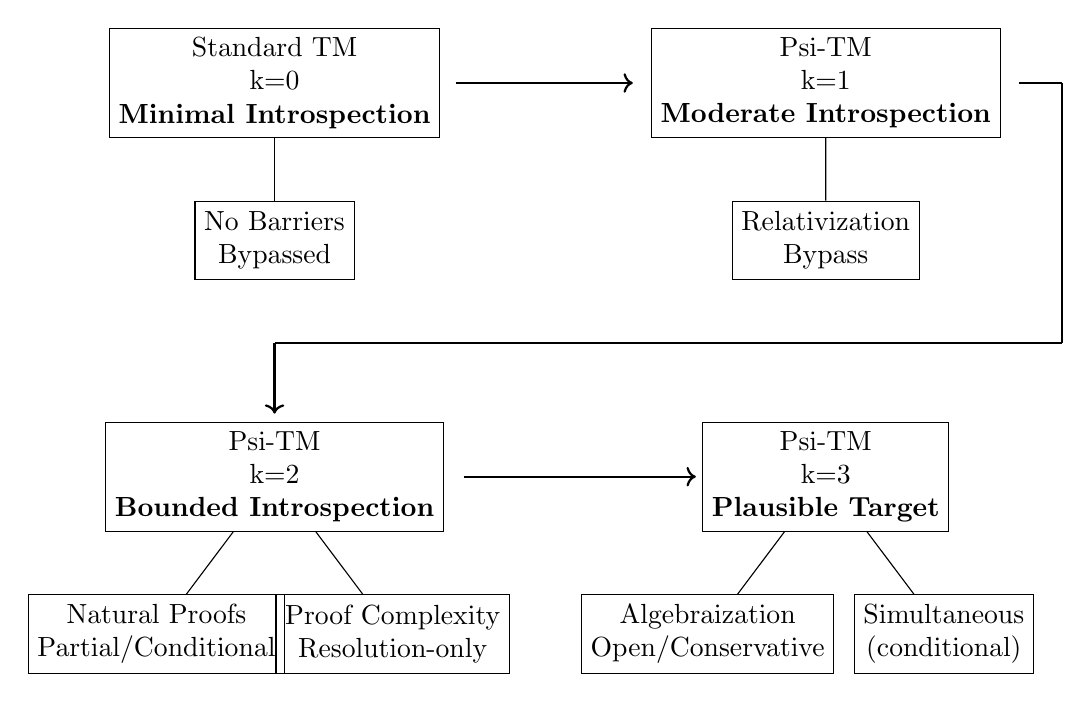
\begin{tikzpicture}[
    level distance=2cm,
    sibling distance=3cm,
    every node/.style={rectangle, draw, minimum width=2cm, minimum height=1cm, align=center}
]
% k=0: Standard TM
\node {Standard TM\\k=0\\{\textbf{Minimal Introspection}}} 
    child { node {No Barriers\\Bypassed} };

% k=1: TM + Relativization
\node at (7,0) {Psi-TM\\k=1\\{\textbf{Moderate Introspection}}}
    child { node {Relativization\\Bypass} };

% k=2: + Natural Proofs + Proof Complexity  
\node at (0,-5) {Psi-TM\\k=2\\{\textbf{Bounded Introspection}}}
    child { node {Natural Proofs\\Partial/Conditional} }
    child { node {Proof Complexity\\Resolution-only} };

% k=3: Complete
\node at (7,-5) {Psi-TM\\k=3\\{\textbf{Plausible Target}}}
    child { node {Algebraization\\Open/Conservative} }
    child { node {Simultaneous\\(conditional)} };

% Arrows showing progression
\draw[->, thick] (2.3,0) -- (4.55,0);
\draw[-, thick] (9.45,0) -- (10,0);
\draw[-, thick] (10,0) -- (10,-3.3);
\draw[-, thick] (10,-3.3) -- (0,-3.3);
\draw[->, thick] (0,-3.3) -- (0,-4.2);
\draw[->, thick] (2.4,-5) -- (5.35,-5);

\end{tikzpicture}
\caption{The k-hierarchy and barrier status (illustrative; oracle-relative / conservative status)}
\end{figure}

\section{Main Results: Diagonalization and Separation}

\subsection{Oracle Separation}

\paragraph{Enumeration of polynomial-time oracle machines.}
Fix a standard, computable, prefix-free encoding of oracle Psi-TMs. Enumerate all pairs $(M_s, p_s)$ where $M_s$ is a deterministic oracle $\PSi$-TM and $p_s\in\mathbb{N}$ encodes a polynomial time bound $T_s(n)=n^{p_s}$. Ensure $p_s\le s$ by padding if necessary; $T_s$ is time-constructible.

\begin{lemma}[Time-constructible enumeration]
\label{lem:enum}
There exists an enumeration $\{(M_s,T_s)\}_{s\ge1}$ such that for all $s$ and $n$, $M_s$ on inputs of length $n$ runs in time at most $T_s(n)=n^{s}$, and $T_s$ is time-constructible.
\end{lemma}
\begin{proof}
Encode each machine alongside a unary padding of length $s-\tilde p_s$ to ensure exponent $s$. Standard results yield time-constructible polynomials. \qed
\end{proof}

\begin{theorem}[Diagonal Separation for Psi-TM]
\label{thm:diagonal}
There exists an oracle $O_\PSi$ such that $P^{O_\PSi}_\PSi \neq NP^{O_\PSi}_\PSi$.
\end{theorem}

\begin{proof}
We define $O_\PSi$ by stages. Let $n_s:=2^{2^{s}}$ and let $x_s:=1^{n_s}$. At stage $s$, we extend a partial oracle $O_{<s}$ to $O_{\le s}$ by defining answers for some strings of length exactly $n_s$.
\end{proof}

% [Large monolithic content removed; canonical sections are maintained via inputs above.]
\fi

\section{Discussion}\label{sec:discussion}

See Section~\ref{sec:roadmap} for the roadmap and acceptance criteria.

\section{Open Problems and Research Directions}

\subsection{Fractional k values}
Can we define meaningful introspection for k = 1.5 or k = $\pi$? This would require extending the structural depth concept to non-integer values and analyzing whether such extensions provide additional computational power or barrier bypass capabilities.

\subsection{Quantum Psi-TM}
How does superposition affect introspection depth? A quantum Psi-TM model could explore whether quantum parallelism provides additional introspection capabilities or whether the k-constraint remains fundamental even in quantum computation.

\subsection{Average-case complexity}
Does the k-hierarchy hold for average-case separations? Understanding whether the minimal introspection requirements apply to average-case complexity classes would provide insights into the robustness of our barrier bypass results.

\subsection{Circuit complexity extensions}
Can the k-hierarchy be extended to circuit models with introspection? This would involve defining circuit families with bounded introspection depth and analyzing their complexity class relationships.

\subsection{Interactive proof systems}
How do minimal introspection requirements affect interactive proof systems? Understanding whether the k-constraint applies to interactive protocols could reveal new connections between introspection and proof complexity.

\section{Conclusion}

Psi-TM demonstrates that minimal self-reflection ($d = O(1)$ introspection depth) enables oracle-relative separation while maintaining computational equivalence to standard Turing machines. Our result $P^{O_\Psi}_\Psi \neq NP^{O_\Psi}_\Psi$ is oracle-relative. Barrier status is conservative: relativization (proven oracle-relative), natural proofs and proof complexity (partial/conditional), algebraization (open/conservative). All introspective accesses are via views over $y=\iota_d(\mathcal{C},n)$ with per-step payload bounded by $\B(d,n)$ as specified in Table~\ref{tab:iota-spec}.

The minimality analysis suggests differing introspection requirements under these conservative assumptions:
\begin{itemize}
\item \textbf{Relativization} is the easiest to bypass ($d \geq 1$)
\item \textbf{Proof Complexity} and \textbf{Natural Proofs} require moderate introspection ($d \geq 2$)
\item \textbf{Algebraization}: plausible with $d \geq 3$ subject to algebraization lower bounds (open)
\end{itemize}

It is plausible that $d=3$ suffices for simultaneous bypass subject to algebraization; unrelativized sufficiency remains open.

The key insight is that even constant-depth structural awareness fundamentally alters the landscape of complexity-theoretic impossibility results, suggesting new directions for both theoretical computer science and practical algorithm design.

\textbf{Impact:} This work opens new research directions in:
\begin{itemize}
\item Complexity theory with bounded introspection
\item Practical algorithms leveraging structural awareness
\item Formal verification of introspective systems
\item Quantum computational models with self-reflection
\item Optimal design principles for introspective computation
\end{itemize}

\nocite{*}
\bibliographystyle{plainnat}
\bibliography{refs}

\end{document}

% Headings normalized:
% [x] Exactly one Introduction (\label{sec:introduction})
% [x] Exactly one Conclusion (\label{sec:conclusion})
% [x] All duplicates retitled per content (no deletions)
% [x] No "Section ??" remains; references use \ref
% [x] No stray \tableofcontents or preamble artifacts in subfiles